\documentclass[../notes.tex]{subfiles}

\pagestyle{main}
\renewcommand{\chaptermark}[1]{\markboth{\chaptername\ \thechapter\ (#1)}{}}

\begin{document}




\chapter{Structure Determination}
\section{Intro + Elemental Analysis}
\begin{itemize}
    \item \marginnote{9/4:}Teaching team.
    \begin{itemize}
        \item Prof. Masha Elkin.
        \item Prof. Steve Buchwald.
        \item 8 Teaching Fellows (TFs).
    \end{itemize}
    \item Masha Elkin begins. Steve Buchwald and all TFs introduce themselves. Special roles:
    \begin{itemize}
        \item Head TF: Minh Le.
        \item Electronic TF (contact with questions on Canvas, Piazza, BACON): Angel Garcia-Ramirez.
    \end{itemize}
    \item In this class, you will learn\dots
    \begin{itemize}
        \item New things in organic chemistry;
        \item Old things at a deeper level;
        \item Real-world applications of chemistry.
    \end{itemize}
    \item Why study organic chemistry?
    \begin{itemize}
        \item Chemists manipulate matter, and that's awesome!
        \item By "manipulate matter," we mean making molecules, breaking molecules, making polymers, making detergents, and making sure that all of these things break down in the environment :)
    \end{itemize}
    \item Core questions.
    \begin{itemize}
        \item \emph{How} do we make molecules?
        \item What molecules \emph{should} we make?
    \end{itemize}
    \item Course logistics.
    \begin{itemize}
        \item Seven (7) units total (2 big units before the halfway mark \& 5 smaller units after).
        \item The units.
        \begin{itemize}
            \item Unit 1: How do we know what molecule(s) we have?
            \item Unit 2: How do electrons move?
            \item Units 3-7: How do we make molecules? How do reactions work?
        \end{itemize}
        \item Exams after units 1, 2, 4, and 6; final exam after unit 7.
        \item Questions? Ask your TF first, then the Head TF, then the profs (Masha \& Steve).
    \end{itemize}
    \item Prerequisites.
    \begin{itemize}
        \item Official prerequisites: 5.12 (equivalent to Orgo I, in case you took it elsewhere) \& Gen Chem.
        \item Recommended reading for review: Chapters 1-2 of the main textbook, referred to in these notes as \textcite{bib:Clayden}.
    \end{itemize}
    \item Grading.
    \begin{itemize}
        \item Your grade will (hopefully) be a reflection of your learning.
        \item There are no curves in this class or at MIT, so \emph{everyone can get an A!!!}
        \item How to improve your grade: Do problems!
        \begin{itemize}
            \item Problem sets (PSets) and recitation worksheets will be provided.
            \item You may also do as many textbook problems as you want. Feel free to buy the solutions manual, or borrow a copy from the ChemEd office\footnote{Located in 6-203.} to check your answers.
        \end{itemize}
    \end{itemize}
    \item How to learn organic chemistry.
    \begin{itemize}
        \item Analogy: Learning Orgo is like learning a language.
        \begin{itemize}
            \item Basic vocab and grammar that must be memorized. Examples: Drawing structures, curved arrow formalism, etc.
            \item Recognizing patterns and trends. Examples: Nucleophiles tend to have lone pairs (or be other regions of high electron density).
            \item Developing intuition.
            \item Practice, practice, practice! (Focus on drawing structures.)
        \end{itemize}
        \item Tips for success.
        \begin{itemize}
            \item Be active and participate in lecture, recitation, etc. Take notes while you're here!
            \item Practice \textbf{metacognition}, i.e., learn how you learn.
            \begin{itemize}
                \item Do you learn best in a crowded coffee shop, or in your own room? Would you rather recopy your notes, or read the textbook?
                \item Note that what works for somebody else may not work for you, and vice versa!
                \item Invest the time and effort that \emph{you} need to succeed. This may be more (or less) than other students, and that's ok!
            \end{itemize}
            \item Communicate with \emph{the whole} teaching team. They're here to help!!!
            \begin{itemize}
                \item Seek out accommodations as needed: It's the student's responsibility to ask.
            \end{itemize}
        \end{itemize}
    \end{itemize}
    \item \textbf{Metacognition}: Being aware of your own understanding.
    \item We now begin the content for Unit 1.
    \item Goal: Learn how to determine the chemical structure of a given organic compound.
    \item Why do we need to determine structures?
    \begin{figure}[h!]
        \centering
        \begin{tikzpicture}
            \begin{scope}[xshift=-1cm,scale=0.4]
                \fill [gaz] (-0.5,0) -- (-1,-1) -- (1,-1) -- (0.5,0);
                \draw [gay,thick,decorate,decoration={snake,segment length=4pt,amplitude=0.5pt}] (-0.5,0) -- (0.5,0);
    
                \draw [gray,ultra thick] (-0.3,1) -- (-0.3,0.5) -- (-1,-1) -- (1,-1) -- (0.3,0.5) -- (0.3,1);
            \end{scope}
            \draw [thick,-latex] (-0.4,0) -- (0.4,0);
            \node at (1.1,0) {\chemfig[atom sep=1.4em]{*6(-=-=-=)}};
        \end{tikzpicture}
        \caption{Why we study structure determination.}
        \label{fig:structureDeterminationRationale}
    \end{figure}
    \begin{itemize}
        \item With the naked eye, organic chemists see a flask with a colorless liquid. But we draw the skeletal diagram for benzene (which is a colorless liquid). What tools enable us to convert from the flask to the structure?
        \item Here's another reason: Suppose we run a brand new chemical reaction. Organic chemists do this all the time in research! How do we now what the product is? How do we know which atoms it contains, and in what arrangement?
    \end{itemize}
    \item Structure determination workflow.
    \begin{enumerate}
        \item Identify the atoms present.
        \begin{itemize}
            \item Questions to answer: What is the molecular formula?
            \item Relevant tools: Elemental analysis (EA) and mass spectrometry ("mass spec" or MS).
        \end{itemize}
        \item Identify the functional groups and substructures present.
        \begin{itemize}
            \item Questions to answer: Do we have ketones? Esters? Alcohols? Rings?
            \item Relevant tools: MS, infrared spectroscopy (IR), and nuclear magnetic resonance (NMR).\footnote{NMR is an organic chemist's best friend!}
        \end{itemize}
        \item Identify how all the functional groups fit together.
        \begin{itemize}
            \item Questions to answer: Are they close? Far apart? Ortho/meta/para? What stereochemistry?
            \item Relevant tools: NMR and X-ray diffraction.
        \end{itemize}
    \end{enumerate}
    \item We now begin talking about EA.
    \begin{itemize}
        \item History: Began development in the 1820s.
        \item Purpose: Determine which elements are present, and in what quantities (in a given sample).
    \end{itemize}
    \item In this course, we will apply EA to compounds containing carbon, hydrogen, and oxygen \emph{exclusively}.
    \begin{itemize}
        \item To reiterate, in an EA problem for this course, we will \emph{not} have to worry about any other elements.
        \item The typical EA technique for such compounds is \textbf{combustion analysis}.
    \end{itemize}
    \item \textbf{Combustion analysis}: Burn the sample and measure the products.
    \begin{itemize}
        \item All \ce{C} in the sample becomes \ce{CO2}.
        \item All \ce{H} in the sample becomes \ce{H2O}.
        \item \ce{O} is then determined via process of elimination, explained as follows.
    \end{itemize}
    \item Advanced techniques (beyond the scope of this class): Nitrogen to \ce{NO} or \ce{NO2}, sulfur to \ce{SO2}, etc.
    \item A schematic of combustion analysis.
    \begin{figure}[h!]
        \centering
        \begin{tikzpicture}
            \footnotesize
            \filldraw [draw=brown,thick,fill=brown!20] (0,-0.18) ellipse (2mm and 1mm);
            \node at (0,0.8) {Sample}
                edge[bend right=10,->] (0,0)
            ;
            \node at (0,-0.8) {\ce{CuO}}
                edge[bend right=10,->] (0.5,-0.1)
            ;
    
            \fill [gaz] (1.4,-1)
                -- ({1.4+0.24},-1)
                arc[start angle=-140,end angle=-40,x radius=0.73cm,y radius=1.12cm]
                -- ({1.4+1.6},-1)
                arc[start angle=-40,end angle=-140,x radius=1.04cm,y radius=1.66cm]
                -- cycle
            ;
            \draw [gay,thick,decorate,decoration={snake,segment length=4pt,amplitude=0.5pt}] (1.4,-1) -- (1.64,-1);
            \draw [gay,thick,decorate,decoration={snake,segment length=4pt,amplitude=0.5pt}] (2.76,-1) -- (3,-1);
            \node at (2.2,-2.1) {\ce{CaCl2}}
                edge[bend right=10,->] (2.2,-1.45)
            ;
            \fill [gaz] (3.5,-1)
                -- ({3.5+0.24},-1)
                arc[start angle=-140,end angle=-40,x radius=0.73cm,y radius=1.12cm]
                -- ({3.5+1.6},-1)
                arc[start angle=-40,end angle=-140,x radius=1.04cm,y radius=1.66cm]
                -- cycle
            ;
            \draw [gay,thick,decorate,decoration={snake,segment length=4pt,amplitude=0.5pt}] (3.5,-1) -- ({3.5+0.24},-1);
            \draw [gay,thick,decorate,decoration={snake,segment length=4pt,amplitude=0.5pt}] ({3.5+1.6-0.24},-1) -- ({3.5+1.6},-1);
            \node at (4.3,-2.1) {\ce{KOH}}
                edge[bend right=10,->] (4.3,-1.45)
            ;
    
            \draw
                (-1.2,0) ellipse (0.5mm and 1mm)
                (-1.2,0.1)  -- (-0.7,0.1)
                (-1.2,-0.1) -- (-0.7,-0.1)
                (-0.7,-0.3) rectangle (0.7,0.3)
                (0.7,-0.1) -- (1.2,-0.1)
                    arc[start angle=-180,end angle=0,x radius=1cm,y radius=1.5cm]
                    -- ++(0.1,0)
                    arc[start angle=-180,end angle=0,x radius=1cm,y radius=1.5cm]
                    -- ++(0.3,0)
                (0.7,0.1) -- (1.38,0.1)
                    arc[start angle=-180,end angle=0,x radius=0.82cm,y radius=1.5cm]
                    -- ++(0.46,0)
                    arc[start angle=-180,end angle=0,x radius=0.82cm,y radius=1.5cm]
                    -- ++(0.48,0)
                (5.6,0) ellipse (0.5mm and 1mm)
            ;
            \node at (-2,0) {\ce{O2}}
                edge [->] (-1.4,0)
            ;
            \node at (6.4,0) {\ce{O2}}
                edge [<-] (5.8,0)
            ;
        \end{tikzpicture}
        \caption{Combustion analysis schematic.}
        \label{fig:schematicEA}
    \end{figure}
    \begin{itemize}
        \item Burn the sample in the presence of an oxidant such as cupric oxide (\ce{CuO}).
        \item Flow \ce{O2} into the combustion chamber to facilitate burning as well.
        \item The combusted gas then flows through a series of reaction containers.
        \begin{itemize}
            \item The first one contains a desiccant (like \ce{CaCl2}) that absorbs the water.
            \item The second one contains a base (like \ce{KOH}) that absorbs the \ce{CO2}.
        \end{itemize}
        \item The remaining oxygen flows out the end.
    \end{itemize}
    \item The \emph{analysis} part of combustion analysis.
    \begin{itemize}
        \item The amount of \ce{H} is equal to the change in mass of the \ce{CaCl2}.
        \begin{equation*}
            \Delta\text{mass}(\ce{CaCl2}) = \text{mass}(\ce{H2O})
            \to \text{ratio}(\ce{H})
        \end{equation*}
        \item The amount of \ce{C} is equal to the change in mass of the \ce{KOH}.
        \begin{equation*}
            \Delta\text{mass}(\ce{KOH}) = \text{mass}(\ce{CO2})
            \to \text{ratio}(\ce{C})
        \end{equation*}
        \item The amount of \ce{O} is equal to the change in mass of the sample.
        \begin{equation*}
            \text{mass}(\text{sample})-\text{mass}(\ce{H})-\text{mass}(\ce{C}) = \text{mass}(\ce{O})
             \to \text{ratio}(\ce{O})
        \end{equation*}
        \item Result: We get an \textbf{empirical formula} of the form \ce{C_{$x$}H_{$y$}O_{$z$}}. Remember that this is \emph{not} (necessarily) the \textbf{molecular formula}; it is \emph{only} a ratio of elements.
    \end{itemize}
    \item EA example: Let's burn \SI{0.5}{\gram} of propanol (\ce{C3H8O}).
    \begin{itemize}
        \item Suppose we obtain \SI{0.600}{\gram} \ce{H2O} and \SI{1.09}{\gram} \ce{CO2}.
        \item This means that there was \SI{0.067}{\gram} (\ce{H}) and \SI{0.300}{\gram} (\ce{C}) in the sample. The remaining \SI{0.133}{\gram} must then be due to \ce{O}.
        \item Therefore, the elements exist in a 3:8:1 (C:H:O) ratio.
        \item Bonus: Convert the masses to a ratio via stoichiometry.
        \begin{itemize}
            \item $
                \SI{0.600}{\gram}\ \ce{H2O}
                \times\dfrac{\SI{1}{\mole}\ \ce{H2O}}{\SI{18.02}{\gram}\ \ce{H2O}}
                \times\dfrac{\SI{2}{\mole}\ \ce{H}}{\SI{1}{\mole}\ \ce{H2O}}
                \times\dfrac{\SI{1.01}{\gram}\ \ce{H}}{\SI{1}{\mole}\ \ce{H}}
                = \SI{0.067}{\gram}\ (\ce{H})
            $
            \item $
                \SI{1.09}{\gram}\ \ce{CO2}
                \times\dfrac{\SI{1}{\mole}\ \ce{CO2}}{\SI{44.01}{\gram}\ \ce{CO2}}
                \times\dfrac{\SI{1}{\mole}\ \ce{C}}{\SI{1}{\mole}\ \ce{CO2}}
                \times\dfrac{\SI{12.01}{\gram}\ \ce{C}}{\SI{1}{\mole}\ \ce{C}}
                = \SI{0.300}{\gram}\ (\ce{C})
            $
            \item $
                \SI{0.5}{\gram}\ \text{propanol}
                -\SI{0.067}{\gram}\ (\ce{H})
                -\SI{0.300}{\gram}\ (\ce{C})
                = \SI{0.133}{\gram}\ (\ce{O})
            $
        \end{itemize}
    \end{itemize}
    \item A note on the previous example.
    \begin{table}[h!]
        \centering
        \small
        \renewcommand{\arraystretch}{1.4}
        \begin{tabular}{l|cc|ccc}
            \textbf{Name} & Propanol & Methyl ethyl ether & Formaldehyde & Acetic acid & Glucose\\
            \textbf{Structure} &
                \footnotesize\chemfig[atom sep=1em]{-[:30]-[:-30]-[:30]OH} &
                \footnotesize\chemfig[atom sep=1em]{-[:30]-[:-30]O-[:30]} &
                \footnotesize\chemfig[atom sep=1em,baseline=1.2em]{H-[:30](=[2]O)-[:-30]H} &
                \footnotesize\chemfig[atom sep=1em,baseline=0.65em]{-[:30](=[2]O)-[:-30]OH} &
                \footnotesize\chemfig[atom sep=1em,baseline=-0.4em]{?(-[:190]HO)-[:-50,1.4](-[:170]HO)-[:10,1.5](-[:-55]OH)-[:-10,1.5](-[:10]OH)-[:130]O-[:190]?(-[:150,0.7]-[2]OH)}\\
            \textbf{Emp. formula} & \ce{C3H8O} & \ce{C3H8O} & \ce{CH2O} & \ce{CH2O} & \ce{CH2O}\\
            \textbf{Mol. formula} & \ce{C3H8O} & \ce{C3H8O} & \ce{CH2O} & \ce{C2H4O2} & \ce{C6H12O6}\\
        \end{tabular}
        \caption{Questions that EA can't answer.}
        \label{tab:EAmols}
    \end{table}
    \begin{itemize}
        \item EA has given us the empirical formula, but it has \emph{not} confirmed that the sample is propanol. For example, methyl ethyl ether has the same empirical formula!
        \item Additionally, we don't yet have the molecular formula. Consider, for instance, the breadth of compounds with empirical formula \ce{CH2O}!
        \item Takeaway: EA gives you the empirical formula; we need MS to get the molecular formula (we'll see this on Friday), and we may need even more to get the atomic connectivity.
    \end{itemize}
    \item Application of EA to real-world chemistry.
    \begin{itemize}
        \item A home furnace burns natural gas --- which is mostly methane (\ce{CH4}) --- for heat.
        \item \textbf{Ideal combustion}\footnote{You can learn more about in a chemical engineering/ChemE course.} corresponds to the reaction
        \begin{equation*}
            \ce{CH4 + O2 -> CO2 + H2O}
        \end{equation*}
        \item Real-world combustion is incomplete; you make
        \begin{equation*}
            \ce{CH4 + air -> CO2 + H2O + NO2 + CO}
        \end{equation*}
        \item When a technician comes to your home, they analyze the flue gas (i.e., your furnace exhaust).
        \begin{itemize}
            \item Their analysis could determine that our combustion has too much \ce{O2}, which is called "air rich." This is inefficient and doesn't yield enough heat.
            \item They could also determine that you have too much \ce{CO2} and \ce{CO}, which is called "fuel rich." This yields too much soot and \ce{CO}. \ce{CO} can be dangerous and lead to carbon monoxide poisoning, which makes you sleepy before it kills you.
        \end{itemize}
        \item To measure this flue gas, though, they have a little handheld elemental analysis device!
    \end{itemize}
    \item Note that there is a relation between ideal/real-world combustion and the \ce{CuO} oxidant in Figure \ref{fig:schematicEA}: The \ce{CuO} ensures that when we combust our EA sample, all the carbon is fully oxidized to \ce{CO2}! Without it, some \ce{CO} would be formed, and our stoichiometry would be thrown off.
\end{itemize}



\section{Mass Spectrometry}
\begin{itemize}
    \item \marginnote{9/6:}Lecture 1 recap.
    \begin{itemize}
        \item Elemental analysis (EA).
        \begin{equation*}
            \ce{SM + O2 ->[$\Delta$] CO2 + H2O}
        \end{equation*}
        \begin{itemize}
            \item SM means "\underline{s}tarting \underline{m}aterial."
            \item SM's we will focus on: Compounds of the form \ce{C_{$x$}H_{$y$}O_{$z$}}.
        \end{itemize}
        \item Empirical formula vs. molecular formula (see Table \ref{tab:EAmols}).
    \end{itemize}
    \item Today: Mass spectrometry (MS).
    \begin{itemize}
        \item Purpose: Convert empirical formulas to molecular formulas (and more!).
        \item Reading: \textcite{bib:Clayden}, Chapter 3.
    \end{itemize}
    \item Lecture outline.
    \begin{itemize}
        \item Mass spectrometer schematic.
        \item Mass spectrum elements.
        \item Fragmentation, and common types.
        \item Isotope effects in MS.
        \item Ionization methods.
    \end{itemize}
    \item \textbf{Mass spectrometry}: A structure determination technique that tells us the exact mass of molecules and their "fragments." \emph{Also known as} \textbf{MS}, "\textbf{mass spec}."
    \item Overview.
    \begin{center}
        \schemestart
        \chemfig{\cnc{M}}
        \arrow{-U>[\footnotesize$\textup{e}^-$][\footnotesize$2\textup{e}^-$]}
        \chemfig{\charge{20=\scriptsize +,-3=$\cdot$}{\cnc{M}}}
        \arrow(M--b)
        \subscheme{
            \chemfig{\charge{12=\scriptsize +}{\cnc{M$-b$}}}
            \+{3mm}
            \chemfig{\charge{[extra sep=1pt]30=$\cdot$}{\cnc{$b$}}}
        }
        \arrow(--a){0}[90,0.1]
        \subscheme{
            \chemfig{\charge{12=\scriptsize +}{\cnc{M$-a$}}}
            \+{3mm}
            \chemfig{\charge{[extra sep=1pt]30=$\cdot$}{\cnc{$a$}}}
        }
        \arrow(@b--c){0}[-90,0.1]
        \subscheme{
            \chemfig{\charge{12=\scriptsize +}{\cnc{M$-c$}}}
            \+{3mm}
            \chemfig{\charge{[extra sep=1pt]30=$\cdot$}{\cnc{$c$}}}
        }
        \arrow(@M--@a.west)
        \arrow(@M--@c.west)
        \schemestop
    \end{center}
    \begin{itemize}
        \item You have a sample --- denoted by $\cnc{M}$ --- that you bombard with electrons ($\e[-]$). When an electron hits a molecule of your sample, it knocks off one of the molecule's electrons (and flies off itself). This ionizes your molecule to a \textbf{radical cation}, denoted by $\cnc{M}\rc$ and called the \textbf{molecular ion}.
        \item This radical cation is unstable and fragments into a proper cation and a proper radical. The radical is usually not detected, but any cationic fragment produced --- the $\cnc{M$-a$}^+$, $\cnc{M$-b$}^+$, and $\cnc{M$-c$}^+$ above --- usually \emph{is} detected.
    \end{itemize}
    \item A (stepwise) schematic of a mass spectrometer.
    \begin{figure}[h!]
        \centering
        \footnotesize
        \begin{tikzpicture}
            \fill [gray!70,rotate around={-10:(2.3,0)}] (1.8,-0.8)
                -- node[below=1mm,black,digit]{5} (2.8,-0.8)
                -- (2.8,0.6)
                -- (1.8,0.6)
            ;
            \fill [white] (-0.3,0.1)
                -- (0,0.1)
                -- (0,0.5)
                -- (1.5,0.5)
                arc[start angle=90,end angle=35,radius=4cm]
                -- ++(-145:1)
                arc[start angle=35,end angle=90,radius=3cm]
                -- (0,-0.5)
                -- (0,-0.1)
                --(-0.3,-0.1)
            ;
    
            \draw [decorate,decoration={coil,segment length=2.2pt},rotate around={180:(0.4,0.4)}] (0.1,0.4) -- node[above=2mm,digit]{2} (0.7,0.4);
    
            \draw (0.2,-0.5)
                -- (0.2,-0.9)
                -- node[below=1mm,digit]{3} (0.5,-0.9)
                -- (0.5,-0.5)
            ;
            \draw [-stealth] (0.35,-0.45) -- ++(0,0.23);
            \draw [-stealth] (0.42,-0.45) -- ++(0.12,0.16);
            \draw [-stealth] (0.28,-0.45) -- ++(-0.12,0.16);
    
            \draw
                (-0.3,0) ellipse (0.3mm and 1mm)
                (-0.3,0.1) -- (0,0.1)
                    -- (0,0.5)
                    -- (1.5,0.5)
                    arc[start angle=90,end angle=35,radius=4cm] coordinate (b) node[right=1mm,digit]{6}
                (-0.3,-0.1) -- (0,-0.1)
                    -- (0,-0.5)
                    -- (1.5,-0.5)
                    arc[start angle=90,end angle=35,radius=3cm] coordinate (a) %node[left=2mm,digit]{6}
            ;
            \draw
                (1,0.5) arc[start angle=90,end angle=-90,x radius=1mm,y radius=5mm]
                (1.3,0.5) arc[start angle=90,end angle=-90,x radius=1mm,y radius=5mm]
                (0.9,0.02)  -- ++(0.2,0)
                (0.9,-0.02) -- ++(0.2,0)
                (1.2,0.02)  -- ++(0.2,0)
                (1.2,-0.02) -- ++(0.2,0)
            ;
            \draw
                (1,0.5) arc[start angle=90,end angle=270,x radius=1mm,y radius=5mm]
                (1.3,0.5) arc[start angle=90,end angle=270,x radius=1mm,y radius=5mm]
            ;
            \node [below,digit] at (1.15,-0.6) {4};
            \draw [rotate=-55] ($(a)!0.5!(b)+(0,0.5)$) arc[start angle=90,end angle=-90,x radius=1mm,y radius=5mm];
            \draw [rotate=-55] ($(a)!0.5!(b)+(0,0.5)$) arc[start angle=90,end angle=270,x radius=1mm,y radius=5mm];
    
            \node [label={[above,digit]1}] at (-1.8,0) {Sample}
                edge [dashed,->] (-0.45,0)
            ;
            \draw [dashed,->] (-0.1,0) -- (0.85,0);
            \draw [dashed,->] (1.45,0)
                -- (1.5,0)
                arc[start angle=90,end angle=49,radius=1.9cm] %node[circle,fill,inner sep=1pt]{}
                -- ++({49-90}:1.65)
            ;
            \draw [dashed,->] (1.45,0)
                -- (1.5,0)
                arc[start angle=90,end angle=57,radius=2.3cm] %node[circle,fill,inner sep=1pt]{}
                -- ++({57-90}:1.8)
            ;
            \draw [dashed,->] (1.45,0)
                -- (1.5,0)
                arc[start angle=90,end angle=63,radius=2.8cm] %node[circle,fill,inner sep=1pt]{}
                -- ++({63-90}:1.93)
            ;
        \end{tikzpicture}
        \caption{Mass spectrometer schematic.}
        \label{fig:schematicMS}
    \end{figure}
    \begin{enumerate}
        \item The sample is injected into a curved tube.
        \item A heater vaporizes the sample.
        \item An electron source (also known as an electron gun) shoots electrons at the vaporized sample, ionizing it. The ionized sample starts fragmenting.
        \item The fragments encounter a series of negatively charged plates with slits in the middle. These negatively charged plates accelerate the positively charged cations.
        \item A magnet deflects the accelerated, positively charged ions. The magnet deflects them based on their \textbf{mass-to-charge ratio}. Because of physics, the lightest ions are deflected the most, and the heaviest ions are deflected the least.
        \item A detector records where the ions hit. This data is converted into a mass-to-charge ratio for each ion. This yields a spectrum of all the fragments' masses.
    \end{enumerate}
    \item \textbf{Mass-to-charge ratio} (of a cation): The cation's mass divided by its net charge. \emph{Denoted by} $\bm{m/z}$.
    \begin{itemize}
        \item For the purposes of this class, $z=1$.
    \end{itemize}
    \item Example mass spectrum: Acetone (\,{\tiny\chemfig[baseline=1mm,atom sep=1em,bond offset=1pt,fixed length=false]{-[:30](=[2]O)-[:-30]}}\,).
    \begin{figure}[H]
        \centering
        \begin{tikzpicture}[xscale=0.16,yscale=0.04]
            \small
            \node [rotate=90] at (-5.875,50) {Relative Intensity};
            \node [below=5mm] at (35,0) {$m/z$};
    
            \footnotesize
            \draw (-0.625,100) node[left]{$100$} -- ++(1.125,0);
            \foreach \x in {10,20,...,60} {
                \draw (\x,2.5) -- ++(0,-5) node[below]{$\x$};
            }
    
            \draw [orange,ultra thick]
                (15,0) -- ++(0,14) node[above=1mm,black,thin,digit]{15} node[above=6mm,black]{$\cnc{M$-43$}^+=\cnc{CH3}^+$}
                (27,0) -- ++(0,1)
                (28,0) -- ++(0,1)
                (29,0) -- ++(0,1)
                (43,0) -- ++(0,100) node[above=1mm,black,thin,digit]{43} node[above=6mm,black]{${}^{\color{white}+}\cnc{M$-15$}^+=[\chemfig[atom sep=1.4em,fixed length=false,bond sep=2pt]{H_3C-~O}]^+$}
                (44,0) -- ++(0,3)
                (58,0) -- ++(0,26) node[above=1mm,black,thin,digit]{58} node[above=6mm,black]{${}^{\color{white}+}\cnc{M}\rc=\Big[{\tiny\chemfig[baseline=1.3mm,atom sep=1em,bond offset=1pt,fixed length=false]{-[:30](=[2]O)-[:-30]}}\Big]{}^\rc$}
                (59,0) -- ++(0,2)
            ;
    
            \draw (0,110) -- (0,0) -- (70,0);
        \end{tikzpicture}
        \vspace{-0.5em}
        \caption{Mass spectrum of acetone.}
        \label{fig:MSacetone}
    \end{figure}
    \begin{itemize}
        \item The $x$-axis is the mass-to-charge ratio, and the $y$-axis is the "relative intensity" of each peak.
        \begin{itemize}
            \item If a certain fragment gets produced more than another (and hence recorded more than it), we say it has a "higher relative intensity."
        \end{itemize}
        \item We identify two special types of peaks in a mass spectrum: The \textbf{parent peak} and the \textbf{base peak}. In the case of acetone\dots
        \begin{itemize}
            \item The parent peak lies at 58;
            \item The base peak lies at 43.
        \end{itemize}
        \item The peak at 15 also has a relatively large magnitude, and from the fact that the mass of a methyl cation is approximately 15, we can infer that this peak corresponds to the methyl cation fragment.
        \begin{itemize}
            \item Notice that its intensity is significantly lower than the intensity of the base peak because we may recall from Orgo I that the methyl cation is a far less stable cation than the resonance-stabilized, secondary acylium ion at 43.
        \end{itemize}
        \item There are a number of smaller peaks, too, but they give less information.
        \item Note that the major peaks may be appropriately referred to by \emph{any} of the three nomenclature methods in Figure \ref{fig:MSacetone}: By exact mass, by $\cnc{M$-a$}^+$, and/or by structure.
    \end{itemize}
    \item \textbf{Parent peak}: The peak in a mass spectrum corresponding to the molecular ion.
    \begin{itemize}
        \item The parent peak is always the rightmost peak in the spectrum.\footnote{Excepting isotope effects; discussed later in this lecture.} This is because it is created by the heaviest ion, and you can't have more mass than your initial molecule!
        \item It is typically \emph{not} the tallest peak in the spectrum.
        \item Useful information: It gives the molecular weight of the molecule.
    \end{itemize}
    \item \textbf{Base peak}: The tallest peak in a mass spectrum.
    \begin{itemize}
        \item The base peak corresponds to the fragment that the molecule forms most preferentially, which is usually also the most stable fragment.
    \end{itemize}
    \item \textbf{Fragmentation peak}: Any peak to the left of the parent peak.
    \item Maxim: Molecules fragment in predictable ways to form stable cations.
    \item At this point, let's formally define \textbf{fragmentation}.
    \item \textbf{Fragmentation}: The formation of stable(-ish) cations.
    \begin{itemize}
        \item Recall from Orgo I (review your notes on cation stability!!) that stable cations tend to be more substituted, delocalized, atom-stabilized (e.g., close to a heteroatom), etc. 
    \end{itemize}
    \item Let's now discuss some common species that we analyze via MS --- and how they fragment.
    \item Alkane fragmentation: Preferentially break bonds to get more substituted (e.g., $2^\circ$ \& $3^\circ$) carbocations.
    \item Example: Isopentane (\,{\tiny\chemfig[baseline=0.8mm,atom sep=1em,bond offset=1pt,fixed length=false]{-[:30](-[2])-[:-30]-[:30]}}\,).
    \begin{figure}[H]
        \centering
        \footnotesize
        \setchemfig{atom sep=1.4em}
        \schemestart
            \chemfig{-[:30](-[@{1}2])-[@{2}:-30]-[:30]}
            \arrow(--.174)
            \chemname{
                \chemleft[
                    \chemfig{-[:30](-[2])-[:-30]-[:30]}
                \chemright]
            }{$m/z=72$\\parent (minor)}
            \+{,,2mm}
            \chemname{
                \chemleft[
                    \chemfig{-[:30]\charge{[extra sep=5pt]90=$\oplus$}{}(-[2,,,,opacity=0])-[:-30]-[:30]}
                \chemright]
            }{$m/z=57$\\(major)}
            \+{,,2mm}
            \chemname{
                \chemleft[
                    \chemfig{-[:30]\charge{[extra sep=4pt]-30=$\oplus$}{}(-[2])-[:-30,,,,opacity=0]}
                \chemright]
            }{$m/z=43$\\(major)}
            \arrow{0}[,0.1]\+{,,2.5em}\arrow(--.165){0}[0,0.1]
            \chemname[1.2em]{
                \chemleft[
                    \chemfig{Et}
                \chemright]
            }{$m/z=29$\\(minor)}
            \arrow{0}[,0.1]\+{,,3.43em}\arrow{0}[0,0.1]
            \chemname[1.2em]{
                \chemleft[
                    \chemfig{Me}
                \chemright]
            }{$m/z=15$\\(minor)}
        \schemestop
        \hspace{-2mm}
        \chemmove{
            \draw [-,rex] ($(1)+(180:0.18)$) node[circle,draw,fill=white,inner sep=1pt]{} -- ($(1)+(0:0.18)$) node[circle,draw,fill=white,inner sep=1pt]{};
            \draw [-,rex] ($(2)+(-120:0.18)$) node[circle,draw,fill=white,inner sep=1pt]{} -- ($(2)+(60:0.18)$) node[circle,draw,fill=white,inner sep=1pt]{};
        }
        \begin{tikzpicture}[remember picture,overlay]
            % \draw (-13,0.37) -- ++(13,0);
            % \draw (-13,-0.19) -- ++(13,0);
            \node at (-8.82,0.65) {\tiny$\rc$};
            \node at (-1.96,0.38) {${}^+$};
            \node at (0,0.38) {${}^+$};
        \end{tikzpicture}
        \caption{Fragmentation of alkanes.}
        \label{fig:fragAlkane}
    \end{figure}
    \begin{itemize}
        \item All these peaks will appear, but the tallest will correspond to the species labeled "major" above.
    \end{itemize}
    \item Alcohol fragmentation.
    \begin{itemize}
        \item Dehydration: Yields an $\cnc{M$-18$}^+$ peak, corresponding to the loss of water.
        \item $\alpha$-cleavage: Leads to a resonance-stabilized product.
    \end{itemize}
    \item Example: Pentan-3-ol (\,{\tiny\chemfig[baseline=1mm,atom sep=1em,bond offset=1pt,fixed length=false]{(-[:150])-[:30](-[2]OH)-[:-30]-[:30]}}\,).
    \begin{figure}[h!]
        \centering
        \footnotesize
        \setchemfig{atom sep=1.4em}
        \begin{subfigure}[b]{0.49\linewidth}
            \centering
            \schemestart
                \chemname{
                    \chemfig{-[:-30]-[:30](-[@{1}2]OH)-[:-30]-[:30]}
                }{$m/z=88$}
                \arrow
                \chemname{
                    \chemleft[
                        \chemfig{-[:-30]-[:30](-[2,,,,opacity=0]\phantom{OH})=_[:-30]-[:30]}
                    \chemright{]^+}
                }{$m/z=70$}
            \schemestop
            \chemmove{
                \draw [-,rex] ($(1)+(180:0.18)$) node[circle,draw,fill=white,inner sep=1pt]{} -- ($(1)+(0:0.18)$) node[circle,draw,fill=white,inner sep=1pt]{};
            }
            \caption{Dehydration.}
            \label{fig:fragOHa}
        \end{subfigure}
        \begin{subfigure}[b]{0.49\linewidth}
            \centering
            \schemestart
                \chemname{
                    \chemfig{-[:-30]-[:30](-[2]OH)-[@{2}:-30]-[:30]}
                }{$m/z=88$}
                \arrow
                \chemname{
                    \chemleft[\subscheme{
                        \chemfig{-[:-30]-[:30]\charge{[extra sep=4pt]-30=$\oplus$}{}-[2]OH}
                        \arrow{<->}
                        \chemfig{-[:-30]-[:30]=^[2]\charge{[extra sep=4pt]180=$\oplus$}{O}H}
                    }\chemright]
                }{$m/z=59$}
            \schemestop
            \chemmove{
                \draw [-,rex] ($(2)+(-120:0.18)$) node[circle,draw,fill=white,inner sep=1pt]{} -- ($(2)+(60:0.18)$) node[circle,draw,fill=white,inner sep=1pt]{};
            }
            \caption{$\alpha$-cleavage.}
            \label{fig:fragOHb}
        \end{subfigure}
        \caption{Fragmentation of alcohols.}
        \label{fig:fragOH}
    \end{figure}
    \item Ketone fragmentation.
    \begin{itemize}
        \item $\alpha$-cleavage: Leads to a resonance-stabilized product, once again.
        \item McLafferty rearrangement: Only happens for ketones with a $\gamma$-proton.
        \begin{itemize}
            \item We select for this type of ketone because in this case, we can form a six-membered transition state. Recall that six-membered transition states are super stable in organic chemistry!
            \item This fragmentation leads to a charged enol (that we see in the spectrum) and an uncharged olefin (that we don't see in the spectrum).
        \end{itemize}
    \end{itemize}
    \item Example: Hexanones.
    \begin{figure}[h!]
        \centering
        \footnotesize
        \setchemfig{atom sep=1.4em}
        \begin{subfigure}[b]{\linewidth}
            \centering
            \schemestart
                \chemname{
                    \chemfig{(-[:-150])-[:-30]-[@{3}:30](=[2]O)-[@{2}:-30]-[:30]}
                }{$m/z=100$}
                \arrow(.11--.174)
                \chemname{
                    \chemleft[
                        \chemfig{(-[:-150])-[:-30]-[:30]~[:30]\charge{[extra sep=5pt]100=$\oplus$}{O}}
                    \chemright]
                }{$m/z=71$}
                \+
                \chemname{
                    \chemleft[
                        \chemfig{(~[:150]\charge{[extra sep=5pt]80=$\oplus$}{O})-[:-30]-[:30]}
                    \chemright]
                }{$m/z=57$}
            \schemestop
            \chemmove{
                \draw [-,rex] ($(2)+(-120:0.18)$) node[circle,draw,fill=white,inner sep=1pt]{} -- ($(2)+(60:0.18)$) node[circle,draw,fill=white,inner sep=1pt]{};
                \draw [-,rex] ($(3)+(-60:0.18)$) node[circle,draw,fill=white,inner sep=1pt]{} -- ($(3)+(120:0.18)$) node[circle,draw,fill=white,inner sep=1pt]{};
            }
            % \begin{tikzpicture}[remember picture,overlay]
            %     \draw (-5,0.88) -- ++(13,0);
            %     \draw (-5,0.32) -- ++(13,0);
            % \end{tikzpicture}
            \caption{$\alpha$-cleavage.}
            \label{fig:fragKetonea}
        \end{subfigure}\\[2em]
        \begin{subfigure}[b]{\linewidth}
            \centering
            \schemestart
                \chemfig{-[:30](=[2]O)-[:-30]\charge{[extra sep=4pt]-90=$\alpha$}{}-[:30]\charge{[extra sep=4pt]90=$\beta$}{}-[:-30]\charge{[extra sep=4pt]-90=$\gamma$}{}-[:30]}
                \arrow(--.170)
                \chemname[0em]{
                    \chemleft[
                        \chemfig[atom sep=2.5em,fixed length=false]{-[:30](=[@{db}2]O)-[@{sb2}:-30]-[@{sb3}:30]-[@{sb4}2](-[@{sb5}:150]H-[@{sb6,0.3}:-150,,,,opacity=0])-[:30]}
                    \chemright]
                }{$m/z=100$}
                \arrow(.10--.151)
                \chemname[1.5em]{
                    \chemleft[
                        \chemfig{-[:30](-[2]OH)=_[:-30]}
                    \chemright]
                }{$m/z=58$}
                \arrow(--.210){0}[,0]\+{,,3.9mm}
                \chemfig{=_[2]-[:30]}
            \schemestop
            \chemmove{
                \draw [curved arrow={2pt}{1pt},arrows={-Stealth[harpoon,flex]}] (db) to[out=10,in=-70,out looseness=2,in looseness=1] (sb6);
                \draw [curved arrow={2pt}{1pt},arrows={-Stealth[harpoon,flex,swap]}] (db) to[out=-10,in=70,out looseness=2,in looseness=1.5] (sb2);
                \draw [curved arrow={1pt}{1pt},arrows={-Stealth[harpoon,flex]}] (sb3) to[out=130,in=50,out looseness=2,in looseness=1.5] (sb2);
                \draw [curved arrow={1pt}{1pt},arrows={-Stealth[harpoon,flex,swap]}] (sb3) to[out=110,in=-170,out looseness=2,in looseness=1.5] (sb4);
                \draw [curved arrow={1pt}{1pt},arrows={-Stealth[harpoon,flex]}] (sb5) to[out=-110,in=170,out looseness=2,in looseness=1.5] (sb4);
                \draw [curved arrow={1pt}{1pt},arrows={-Stealth[harpoon,flex,swap]}] (sb5) to[out=-130,in=-50,out looseness=2,in looseness=1] (sb6);
            }
            \begin{tikzpicture}[remember picture,overlay]
                % \draw (-5,1.45) -- ++(13,0);
                % \draw (-5,0.32) -- ++(13,0);
                \node at (-4.24,1.08) {\tiny$\rc$};
                \node at (-1.12,0.8) {\tiny$\rc$};
            \end{tikzpicture}
            \caption{McLafferty rearrangement.}
            \label{fig:fragKetoneb}
        \end{subfigure}
        \caption{Fragmentation of ketones.}
        \label{fig:fragKetone}
    \end{figure}
    \item Isotope effects.
    \item Principle: Mass spectrometry weighs individual molecules, so molecules containing a heavier (or lighter) isotope will appear separate from other molecules in the mass spectrum.
    \item Atoms with notable isotope effects.
    \begin{figure}[H]
        \centering
        \begin{subfigure}[b]{0.17\linewidth}
            \centering
            \begin{tikzpicture}
                \draw [orange,ultra thick]
                    (0.8,0) -- ++(0,1.2)
                    (0.96,0) -- ++(0,0.05)
                ;

                \draw (0,1.4) -- (0,0) -- (1.8,0);
            \end{tikzpicture}
            \caption{Carbon.}
            \label{fig:isotopeEffectsMSa}
        \end{subfigure}
        \begin{subfigure}[b]{0.17\linewidth}
            \centering
            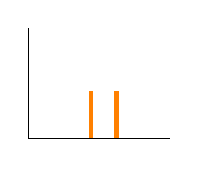
\begin{tikzpicture}
                \draw [orange,ultra thick]
                    (0.8,0) -- ++(0,0.6)
                    (1.12,0) -- ++(0,0.6)
                ;
                
                \draw (0,1.4) -- (0,0) -- (1.8,0);
            \end{tikzpicture}
            \caption{Bromine.}
            \label{fig:isotopeEffectsMSb}
        \end{subfigure}
        \begin{subfigure}[b]{0.17\linewidth}
            \centering
            \begin{tikzpicture}
                \draw [orange,ultra thick]
                    (0.8,0) -- ++(0,0.9)
                    (1.12,0) -- ++(0,0.3)
                ;
                
                \draw (0,1.4) -- (0,0) -- (1.8,0);
            \end{tikzpicture}
            \caption{Chlorine.}
            \label{fig:isotopeEffectsMSc}
        \end{subfigure}
        \caption{Isotope effects in MS.}
        \label{fig:isotopeEffectsMS}
    \end{figure}
    \begin{itemize}
        \item Carbon: The $\ce{{}^12C}:\ce{{}^13C}$ ratio is $99:1$.
        \begin{itemize}
            \item Implication: For every $\cnc{M}\rc$, we see 1\% $\cnc{M$+1$}\rc$.
            \item This is why we see tiny "shadow" peaks to the right of the parent peak and base peak in Figure \ref{fig:MSacetone}!
            \begin{itemize}
                \item Note that the "shadow" of the parent peak is 3\% its height (not 1\%) because there are \emph{three} carbons in the acetone molecular ion.
                \item Similarly, the "shadow" of the base peak is 2\% its height because there are \emph{two} carbons in the acylium ion.
            \end{itemize}
        \end{itemize}
        \item Bromine: The $\ce{{}^79Br}:\ce{{}^81Br}$ ratio is $1:1$.
        \begin{itemize}
            \item Implication: The $\cnc{M}\rc$ and $\cnc{M$+2$}\rc$ peaks exist in a $1:1$ ratio, i.e., have the same height/relative intensity.
            \item The splitting of the molecular ion peak into two such peaks is a super recognizable, distinct, and useful fingerprint of bromine-containing compounds!
        \end{itemize}
        \item Chlorine: The $\ce{{}^35Cl}:\ce{{}^37Cl}$ ratio is $3:1$.
        \begin{itemize}
            \item Implication: The $\cnc{M}\rc$ and $\cnc{M$+2$}\rc$ peaks exist in a $3:1$ ratio.
            \item Similar to bromine, this peak splitting is a fingerprint of chlorine-containing compounds.
        \end{itemize}
    \end{itemize}
    \item Combining everything we've learned up to this point, let's do another example.
    \item Example: Benzyl chloride (\,{\tiny\chemfig[baseline=0.5mm,atom sep=1em,bond offset=1pt,fixed length=false]{*6(=-=(--[:-30]Cl)-=-)}}\,).
    \begin{figure}[h!]
        \centering
        \begin{tikzpicture}[xscale=0.08,yscale=0.04]
            \small
            \node [rotate=90] at (-11.75,50) {Relative Intensity};
            \node [below=5mm] at (80,0) {$m/z$};
    
            \footnotesize
            \draw (-1.25,100) node[left]{$100$} -- ++(2.5,0);
            \foreach \x in {50,100,150} {
                \draw (\x,2.5) -- ++(0,-5) node[below]{$\x$};
            }
    
            \draw [orange,ultra thick]
                (40,0) -- ++(0,8) node[above=1mm,black,thin,digit]{40}
                (65,0) -- ++(0,12) node[above=1mm,black,thin,digit]{65}
                (91,0) -- ++(0,100) node[above=1mm,black,thin,digit,label={[right=2mm,yshift=-2mm,black]
                    \chemleft[
                        \chemfig[atom sep=1em]{*6(=-=(-\charge{[extra sep=5pt]90=$\oplus$}{})-=-)}
                    \chemright]
                }]{91}
                (92,0) -- ++(0,7) node[above right=1mm,black,thin,digit]{92}
                (126,0) -- ++(0,27) node[above=1mm,black,thin,digit,label={[right=2.5mm,yshift=2mm,black]
                    \chemleft[
                        \chemfig[atom sep=1em]{*6(=-=(--[:-30]{}^{35}Cl)-=-)}
                    \chemright{]^\rc}
                }]{126}
                (128,0) -- ++(0,9) node[above right=1mm,black,thin,digit,label={[right=2.5mm,yshift=-2mm,black]
                    \chemleft[
                        \chemfig[atom sep=1em]{*6(=-=(--[:-30]{}^{37}Cl)-=-)}
                    \chemright{]^\rc}
                }]{128}
            ;
    
            \draw (0,110) -- (0,0) -- (160,0);
        \end{tikzpicture}
        \vspace{-0.5em}
        \caption{Mass spectrum of benzyl chloride.}
        \label{fig:MSBnCl}
    \end{figure}
    \begin{itemize}
        \item The parent peak will lie at 126, and the corresponding chlorine isotope peak will lie at 128 and be one-third the height.
        \item The base peak will lie at 91, and the corresponding carbon isotope peak will lie at 92 and be 7\% the height (to account for the 7 carbons in the benzylic cation that may be heavy).
        \begin{itemize}
            \item It will correspond to the most stable fragment, which in this case is the benzylic cation.
            \item The benzylic cation is super stable because its positive charge can be resonance delocalized to four different atoms!
            \item A large peak at $m/z=91$ strongly suggests the presence of an aromatic system.
        \end{itemize}
        \item This example focused on predicting the peaks in a mass spectrum based on reasonable fragmentation patterns. But what if we are given the mass spectrum? What data can we pull out then?
    \end{itemize}
    \item To answer this question, here are some guidelines for the interpretation of mass spectra.
    \item Guidelines for interpretation.
    \begin{itemize}
        \item The parent peak provides the molecular weight of the molecule.
        \begin{itemize}
            \item This allows you to convert an empirical formula obtained from EA to the molecular formula.
        \end{itemize}
        \item The parent peak also reveals key atoms via distinct isotopic fingerprints.
        \begin{itemize}
            \item Examples include bromine and chlorine.
            \item An additional one is the \textbf{nitrogen rule}.
        \end{itemize}
        \item Fragmentation patterns can identify substructures.
        \begin{itemize}
            \item Recall from Lecture 1 (9/4) that identifying substructures is part of the second step of the structure determination workflow!
            \item Common fragments:
            \begin{itemize}
                \item Loss of a methyl group is $-15$.
                \item Loss of an OH group is $-17$.
                \item Loss of \ce{H2O} is $-18$.
                \item Loss of \ce{CO2} is $-44$.
                \item Loss of a \ce{{}^$t$Bu} group is $-57$.
            \end{itemize}
            \item Look at the $m/z$ of the fragments \emph{and} the difference in $m/z$ between certain fragments.
            \begin{itemize}
                \item Example: Maybe a certain fragment is formed by losing both a methyl group \emph{and} water.
            \end{itemize}
        \end{itemize}
        \item Important note: These guidelines are just a guide; we will need multiple forms of evidence to support an assignment.
    \end{itemize}
    \item \textbf{Nitrogen rule}: If you have an odd number of nitrogen in a molecule, you will get an odd molecular weight.
    \begin{itemize}
        \item The basis for this rule lies in the fact that nitrogen is trivalent but has an even mass.
        \begin{itemize}
            \item This means that nitrogen tends to bond an odd number of groups (specifically, 3), making the overall mass odd.
        \end{itemize}
        \item Examples: Ammonia has an odd mass of $17=14+1+1+1$ and methylamine has an odd mass of $31=(14+1+1)+(12+1+1+1)$, while methane has an even mass of $16=12+1+1+1+1$ and ethane has an even mass of $30=(12+1+1+1)+(12+1+1+1)$.
        \item You can read more about the nitrogen rule \href{https://en.wikipedia.org/wiki/Nitrogen_rule}{here}.
        \item Implication: If you see an odd molecular weight, you \emph{might} have a nitrogen present!
    \end{itemize}
    \item Types of ionization.
    \item \textbf{Electron ionization}: A beam of electrons. \emph{Denoted by} \textbf{EI}. \emph{Also known as} \textbf{hard ionization}.
    \begin{itemize}
        \item This is the method we are using in this class.
    \end{itemize}
    \item \textbf{Electrospray ionization}: Forms charged droplets. \emph{Denoted by} \textbf{ESI}. \emph{Also known as} \textbf{soft ionization}.
    \begin{itemize}
        \item ESI causes less fragmentation.
        \item One implication of this is that you observe a larger parent peak.
        \item Another consequence is that ESI can analyze a broader range of compounds via mass spectrometry than EI can, since some sensitive compounds (like proteins) would never survive an electron beam.
        \begin{itemize}
            \item Nobel Prize in Chemistry (2002) for this application of MS to biology!
        \end{itemize}
    \end{itemize}
    \item \textbf{High resolution mass spectrometry}. \emph{Denoted by} \textbf{HRMS}.
    \begin{itemize}
        \item In "normal" low-resolution mass spectrometry (LRMS), both \ce{N2} and \ce{C2H4} have $m/z=28$.
        \item In HRMS, \ce{N2} has $m/z=28.0061$ and \ce{C2H4} has $m/z=28.0314$.
    \end{itemize}
    \item HRMS leads nicely into our application for today!
    \item Application of MS to real-world chemistry: Isotopic signatures.
    \begin{itemize}
        \item Today, you learned that the $\ce{{}^12C}:\ce{{}^13C}$ ratio is $99:1$.
        \begin{itemize}
            \item In reality, this is an \emph{average} value.
            \item The actual ratio of isotopes is globally uneven, and we as humans have mapped it.
        \end{itemize}
        \item Indeed, isotope abundances vary by time and location due to air patterns, etc.
        \item For example, Montana is home to 2\% more \ce{{}^13C} than Florida!
        \item Implication: We can tell if a narcotic is made in the US (and where) or another country based on the isotopic abundance in it.
        \item We can also track where a person, drug, or uranium sample is from.
        \begin{itemize}
            \item Naturally, the government is very interested in this technology :)
        \end{itemize}
        \item You can also tell if a person eats corn or rice because this leads to different ratios of nitrogen isotopes in our bodies.
    \end{itemize}
\end{itemize}



\section{Infrared Spectroscopy}
\begin{itemize}
    \item \marginnote{9/9:}Lecture 2 recap.
    \begin{itemize}
        \item In mass spectrometry, you ionize your sample $\cnc{M}$ to the molecular ion $\cnc{M}\rc$.
        \item $\cnc{M}\rc$ is detected as the parent peak.
        \begin{itemize}
            \item The parent peak provides the molecular weight (MW) of the molecule.
            \item The parent peak also reveals any isotopic signatures.
        \end{itemize}
        \item Many molecular ions --- once formed --- will fragment into cations $\cnc{M$-a$}^+$, $\cnc{M$-b$}^+$, $\cnc{M$-c$}^+$, etc.
        \begin{itemize}
            \item More stable cations are formed more often, resulting in higher relative intensities.
            \item The \emph{most} stable fragment gives rise to the base peak.
        \end{itemize}
        \item Common fragments include those resulting from\dots
        \begin{itemize}
            \item The loss of a methyl group;
            \item The loss of a water molecule;
            \item $\alpha$-cleavage;
            \item The McLafferty rearrangement (for ketones).
        \end{itemize}
    \end{itemize}
    \item Today: Infrared Spectroscopy (IR).
    \begin{itemize}
        \item Reading: \textcite{bib:Clayden}, Chapter 3.
        \item Prof. Elkin highly recommends the section on IR; be sure to read this!!
    \end{itemize}
    \item Lecture outline.
    \begin{itemize}
        \item Spectrometer schematic.
        \item Theory.
        \item Spectrum elements.
        \item Key regions of a spectrum.
    \end{itemize}
    \item Principle: Irradiate a sample with infrared waves and detect where the sample absorbs these waves.
    \begin{itemize}
        \item This technique is useful for identifying certain functional groups, namely those that absorb IR waves well.
    \end{itemize}
    \pagebreak
    \item A schematic of an infrared spectrometer.
    \begin{figure}[h!]
        \centering
        \footnotesize
        \begin{tikzpicture}
            \node [draw,minimum height=9mm] {IR source};
    
            \node at (3,0) {\chemfig[atom sep=1.4em]{-[:15,0.75](=[2]O)-[:-45,0.8]}};
            \draw (2.6,-0.5) -- node[below=3mm]{Sample} ++(0.8,-0.3) -- ++(0,1.4) -- ++(-0.8,0.3) -- cycle;
    
            \draw (5.7,0) ellipse (5mm and 8mm) node[below=9.5mm]{Detector};
    
            \draw [rex,semithick,-latex,decorate,decoration={snake,amplitude=1.5pt,segment length=5pt,post length=1.5mm}] (0.8,0.3) -- ++(0.5,0);
            \draw [rex,semithick,-latex,decorate,decoration={snake,amplitude=1.5pt,segment length=7pt,post length=1.5mm}] (0.8,0.1) -- ++(0.8,0);
            \draw [rex,semithick,-latex,decorate,decoration={snake,amplitude=1.5pt,segment length=9pt,post length=1.5mm}] (0.8,-0.1) -- ++(1.1,0);
            \draw [rex,semithick,-latex,decorate,decoration={snake,amplitude=1.5pt,segment length=11pt,post length=1.5mm}] (0.8,-0.3) -- ++(1.4,0);
    
            \draw [rex,semithick,-latex,decorate,decoration={snake,amplitude=1.5pt,segment length=5pt,post length=1.5mm}] (3.5,0.3) -- ++(0.5,0);
            \draw [rex,semithick,-latex,decorate,decoration={snake,amplitude=1.5pt,segment length=7pt,post length=1.5mm}] (3.5,0.1) -- ++(0.8,0);
            \draw [rex,semithick,-latex,decorate,decoration={snake,amplitude=1.5pt,segment length=11pt,post length=1.5mm}] (3.5,-0.3) -- ++(1.4,0);
        \end{tikzpicture}
        \caption{Infrared spectrometer schematic.}
        \label{fig:schematicIR}
    \end{figure}
    \begin{itemize}
        \item We begin with a source of infrared radiation. This source shoots waves at our sample, which could be a molecule like acetone. The IR waves that the source emits have a range of frequencies.
        \item The sample will absorb certain frequencies, and the frequencies that are not absorbed are detected by a detector. In other words, the director detects the \textbf{transmittance} of the sample.
    \end{itemize}
    \item \textbf{Transmittance}: How much of each frequency of radiation passes through the sample.
    \item IR theory.
    \begin{figure}[h!]
        \centering
        \footnotesize
        \begin{subfigure}[b]{0.25\linewidth}
            \centering
            \begin{tikzpicture}
                \node (1) at (0,0) [circle,draw=blx,fill=blz,thick] {$m_1^{}$};
                \node (2) at (2,0) [circle,draw=grx,fill=grz,thick] {$m_2^{}$}
                    edge [decorate,decoration={snake,segment length=6.8pt}] (1)
                ;
            \end{tikzpicture}
            \caption{Springy bonds.}
            \label{fig:IRtheorya}
        \end{subfigure}
        \begin{subfigure}[b]{0.25\linewidth}
            \centering
            \begin{tikzpicture}
                \node (1) at (0,0) [circle,draw=gax,fill=gaz,thick] {\phantom{$m_1^{}$}};
                \node (2) at (2,0) [circle,draw=gax,fill=gaz,thick] {\phantom{$m_1^{}$}}
                    edge [decorate,decoration={snake,segment length=6.8pt}] (1)
                ;
    
                \draw [->] (0.25,0.5) -- ++(-0.5,0);
                \draw [->] (1.75,0.5) -- ++(0.5,0);
            \end{tikzpicture}
            \caption{Stretch.}
            \label{fig:IRtheoryb}
        \end{subfigure}
        \begin{subfigure}[b]{0.25\linewidth}
            \centering
            \begin{tikzpicture}
                \node (1) at (-1.25,0) [circle,draw=gax,fill=gaz,thick] {\phantom{$m_1^{}$}}
                    edge [shorten <=2pt,bend right=10,->,thin] (-0.5,-0.3)
                ;
                \node (2) at (0,0.7) [circle,draw=gax,fill=gaz,thick] {\phantom{$m_1^{}$}}
                    edge [decorate,decoration={snake,segment length=6.8pt}] (1)
                ;
                \node (3) at (1.25,0) [circle,draw=gax,fill=gaz,thick] {\phantom{$m_1^{}$}}
                    edge [decorate,decoration={snake,segment length=6.8pt}] (2)
                    edge [shorten <=2pt,bend left=10,->,thin] (0.5,-0.3)
                ;
            \end{tikzpicture}
            \caption{Bend.}
            \label{fig:IRtheoryc}
        \end{subfigure}
        \caption{Infrared spectroscopy theory.}
        \label{fig:IRtheory}
    \end{figure}
    \begin{itemize}
        \item Fundamental assumption: A chemical bond is like a spring between atoms.
        \begin{itemize}
            \item Recall from Gen Chem that in science, we often call a spring a \textbf{harmonic oscillator}. If you don't quite remember this term, review your Gen Chem notes or Google it!!
        \end{itemize}
        \item Let's dive a bit deeper into this analogy: Imagine we have two different atoms of masses $m_1,m_2$ joined by a "spring," as in Figure \ref{fig:IRtheorya}.
        \begin{itemize}
            \item Just like a real spring, chemical bonds can vibrate in different ways: They can stretch and contract (as in Figure \ref{fig:IRtheoryb}), bend (as in Figure \ref{fig:IRtheoryc}), etc.
            \item All of these different motions are called the \textbf{vibrational modes} of the chemical bonds.
        \end{itemize}
        \item Bonds absorb energy from IR waves when the frequency ($\nu$) of the IR wave matches the frequency of the stretching/bending motion.
        \begin{itemize}
            \item In other words, when you hit the resonance frequency, you absorb energy.
            \item This absorption of energy is detected as the loss of transmittance.
        \end{itemize}
        \item The change in energy between vibrational modes is related to characteristics of the bond as follows.
        \begin{equation*}
            \Delta E \approx \sqrt{\frac{k(m_1+m_2)}{m_1m_2}}
        \end{equation*}
        \begin{itemize}
            \item $k$ is the force constant (proportional to the bond strength).
            \item $m$ is the mass of atom 1 or 2.
            \item Implication: Stronger bonds (i.e., those with larger values of $k$) require more energy (i.e., higher $\nu$ IR waves) to absorb.
            \item Implication: Lighter atoms (i.e., those with lower values of $m$) require more energy (i.e., higher $\nu$ IR waves) to absorb.
        \end{itemize}
        \item One additional requirement: The chemical bond must have a dipole in order to absorb IR waves.
        \begin{itemize}
            \item Example: \ce{C#O} absorbs because \ce{O} is more electronegative than \ce{C}, but \ce{N#N} does not.
        \end{itemize}
    \end{itemize}
    \pagebreak
    \item Questions on IR theory.
    \begin{itemize}
        \item Why do bonds absorb energy \emph{only} when the frequency of the IR waves matches the frequency of the bond's vibration?
        \begin{itemize}
            \item The answer to this question is beyond the scope of the class, but Prof. Elkin gives the quantum mechanical explanation.
            \item Essentially, when a chemical bond absorbs energy, it gets excited to a higher-energy vibrational mode, which we may think of as a more intense vibration.
            \item However, because vibrational modes are separated by a set amount of energy, lower energy photons won't have enough energy to make it to the next vibrational mode while higher energy photons will provide too much energy to reach anything stable.
        \end{itemize}
        \item Why don't bonds without dipoles absorb IR waves?
        \begin{itemize}
            \item The explanation is also quantum mechanical, and hence also beyond the scope of this class.
            \item Essentially, symmetric bonds and molecules lack something called a dipole moment, and zero dipole moment zeroes out the absorption in the math of quantum mechanics. 
            \item Note that there is some really cool math and physics underlying the answer to this question, and Prof. Elkin recommends you look it up if you're interested!!
            \item In organic chemistry, however, we're more interested in what we can do with IR spectroscopy than in \emph{exactly} how it works. Essentially, for this class, you should learn how it works well enough to make sense of the trends in spectrum interpretation presented in this lecture, but you don't need to go deeper than that for now.
        \end{itemize}
        \item Why do lighter atoms require more energy? It seems like it would take more energy to push around a heavier atom.
        \begin{itemize}
            \item Check out the explanation in \textcite{bib:Clayden}; it's pretty comprehensive and understandable.
        \end{itemize}
    \end{itemize}
    \item Example IR spectrum: Propionic acid (\,{\tiny\chemfig[baseline=-0.5mm,atom sep=1em,bond offset=1pt,fixed length=false]{-[:-30]-[:30](=[2]O)-[:-30]OH}}\,).
    \begin{figure}[h!]
        \centering
        \begin{tikzpicture}[text height=1.5ex,text depth=0.25ex,xscale=1]
            \small
            \draw (0,4) -- node[rotate=90,above=6mm]{Transmittance (\%)} (0,0) -- node[below=4.7mm]{$\nu$ (\si{\per\centi\meter})} (14,0);
    
            \draw [|-]  (0 ,-1.9) -- node[below=1mm,draw]{\ce{X-H}} ++(6,0);
            \draw [|-]  (6 ,-1.9) -- node[below=1mm,draw]{$sp$} ++(2,0);
            \draw [|-]  (8 ,-1.9) -- node[below=1mm,draw]{\ce{X=Y}} ++(2,0);
            \draw [|-|] (10,-1.9) -- node[below=1mm,draw]{single bonds} ++(4,0);
    
            \footnotesize
            \node [below] at (0,0) {4000};
            \draw (2,0.1)  -- ++(0,-0.1) node[below]{3500};
            \draw (4,0.1)  -- ++(0,-0.1) node[below]{3000};
            \draw (6,0.1)  -- ++(0,-0.1) node[below]{2500};
            \draw (8,0.1)  -- ++(0,-0.1) node[below]{2000};
            \draw (10,0.1) -- ++(0,-0.1) node[below]{1500};
            \draw (12,0.1) -- ++(0,-0.1) node[below]{1000};
            \draw (14,0.1) -- ++(0,-0.1) node[below]{500};
            \draw (0,3.5) -- ++(-0.1,0) node[left]{100};
    
            \draw [<-] (0,-0.6) -- node[below=3mm,align=center]{Higher $E$\\(stronger bonds)} ++(2.3,0);
            \draw [<-] (14,-0.6) -- node[below=3mm,align=center]{Lower $E$\\(weaker bonds)} ++(-2.3,0);
    
            \draw [rex,semithick,decorate,decoration={random steps,segment length=2pt,amplitude=0.8pt},/pgf/fpu/install only={reciprocal}] (0,3.5)
                -- ++(2.5,0)
                to[out=0,in=180,out looseness=0.4,in looseness=0.5] ++(1,-1.7) node[black,above=1.7cm]{\ce{O-H}}
                to[out=0,in=180,out looseness=0.6,in looseness=0.4] ++(0.8,1.7)
                -- ++(3.9,0)
                to[out=0,in=180,out looseness=0.2,in looseness=0.1] ++(0.2,-3.2) node[black,above=3.2cm]{\ce{C=O}}
                to[out=0,in=180,out looseness=0.1,in looseness=0.2] ++(0.2,3.2)
                -- ++(1.2,0)
                to[out=0,in=180,looseness=0.2] ++(0.15,-0.7)
                to[out=0,in=180,looseness=0.5] ++(0.15,0.3) node[black,above=0.4cm]{\ce{C-O}}
                to[out=0,in=180,looseness=0.5] ++(0.15,-1)
                to[out=0,in=180,looseness=0.2] ++(0.15,1.4)
                -- ++(0.3,0)
                to[out=0,in=180,looseness=0.2] ++(0.2,-2) node[black,above=2cm]{\ce{C-O}}
                to[out=0,in=180,looseness=0.2] ++(0.2,2)
                -- ++(0.4,0)
                to[out=0,in=180,looseness=0.8] ++(0.5,-0.6)
                to[out=0,in=180,looseness=0.8] ++(0.3,0.2)
                to[out=0,in=180,looseness=0.8] ++(0.2,-0.1)
                to[out=0,in=180,looseness=0.8] ++(0.4,0.5)
                -- ++(1.1,0)
            ;
        \end{tikzpicture}
        \caption{Infrared spectrum of propionic acid.}
        \label{fig:IRpropionic}
    \end{figure}
    \begin{itemize}
        \item The $x$-axis is the frequency of the IR waves, measured in wavenumbers (\si{\per\centi\meter}).
        \begin{itemize}
            \item We typically are interested in the region from \SIrange{4000}{1500}{\per\centi\meter}.
        \end{itemize}
        \item The $y$-axis is the percent transmittance.
        \item The \textbf{baseline} is 100\%, which means pure transmittance (aka, no \textbf{absorption}).
        \begin{itemize}
            \item Then we have \textbf{absorbance peaks}, each of which corresponds to a different chemical bond.
        \end{itemize}
        \item We can further break the spectrum down into regions.
        \begin{itemize}
            \item \ce{X-H} bonds occur in the \SIrange{4000}{2500}{\per\centi\meter} region.
            \begin{itemize}
                \item Peaks in this region are often broad. Specifically, a peak will be broad if the corresponding protons are \textbf{exchangeable}.
                \item Hydrogen bonding can also lead to broadening.
                \item We see this effect in both IR and NMR, so we'll talk about it more later this week!
                \item For example, the \ce{O-H} peak is broad because this acidic proton is exchangeable.
            \end{itemize}
            \item $sp$-hybridized atoms occur in the \SIrange{2500}{2000}{\per\centi\meter} region.
            \begin{itemize}
                \item In other words, polar triple bonds show up here.
                \item Examples: \ce{C#N} and \ce{C#C$'$}.
            \end{itemize}
            \item \ce{X=Y} bonds occur in the \SIrange{2000}{1500}{\per\centi\meter} region.
            \begin{itemize}
                \item This is for polar double bonds.
                \item Examples: \ce{C=O}, \ce{C=C$'$},\footnote{The prime on the second carbon indicates that the carbons have different substituents. This is necessary if we are to have a dipole (symmetric \ce{C=C} bonds are nonpolar).} and \ce{C=N}.
            \end{itemize}
            \item Single bonds occur in the \SIrange{1500}{500}{\per\centi\meter} region.
            \begin{itemize}
                \item Examples: \ce{C-C$'$}, \ce{C-O}, and \ce{C-F}.
            \end{itemize}
            \item Some of these regions are useful, and some less so.
        \end{itemize}
        \item As you can infer from Figure \ref{fig:IRpropionic}, IR spectra look a bit like icicles.
        \item Note that \ce{C-O} has two peaks because there are multiple bonding modes per bond.
    \end{itemize}
    \item \textbf{Absorption}: The loss of tranmittance.
    \begin{itemize}
        \item We typically plot transmittance in a spectrum, but the two measures are inversely proportional.
    \end{itemize}
    \item \textbf{Exchangeable} (proton): A hydrogen atom that is liable to break off of the rest of the molecule and be replaced by another hydrogen atom in solution.
    \begin{itemize}
        \item This is very much related to acidic protons! Recall that a Br\o nsted acid will donate its proton and then the conjugate base will pick up a new (possibly new) proton all the time. 
    \end{itemize}
    \item \textbf{Diagnostic regions}: \SIrange{4000}{1500}{\per\centi\meter} (useful) and \SIrange{1500}{500}{\per\centi\meter} (useless).
    \item \textbf{Fingerprint region}: The region of an IR spectrum from \SIrange{1500}{500}{\per\centi\meter}.
    \begin{itemize}
        \item Within the fingerprint region, we have so many overlapping peaks that the spectrum becomes difficult to interpret.
        \item However, its shape is characteristic of a molecule, even if it doesn't tell you anything specifically. This is just like a real fingerprint! Your fingerprint doesn't tell anyone else your name, age, date of birth, etc. --- but it does tell people that you're you!
    \end{itemize}
    \item Key regions.
    \begin{table}[H]
        \centering
        \small
        \renewcommand{\arraystretch}{1.4}
        \begin{tabular}{cc|cc|cc}
            \multicolumn{2}{c|}{\textbf{\ce{X-H}}} & \multicolumn{2}{c|}{$\bm{sp}$} & \multicolumn{2}{c}{\textbf{\ce{X=Y}}}\\
            \textbf{FG} & \textbf{$\bm{\nu}$ ($\textbf{cm}^{\bm{-1}}$)} & \textbf{FG} & \textbf{$\bm{\nu}$ ($\textbf{cm}^{\bm{-1}}$)} & \textbf{FG} & \textbf{$\bm{\nu}$ ($\textbf{cm}^{\bm{-1}}$)}\\ \hline
            \ce{O-H} & \numrange{3600}{3200} & \ce{C#N} & \num{2200} & \ce{C=O} & \numrange{1840}{1630}\\
            \ce{N-H} & \numrange{3100}{2700} & \ce{C#C$'$} & \num{2100} & \ce{C=N} & \numrange{1700}{1600}\\
            \ce{C-H} & \numrange{3000}{2850} & \ce{C=C=C$'$} & \num{1950} & \ce{C=C$'$} & \numrange{1670}{1600}\\
        \end{tabular}
        \caption{Key regions of an infrared spectrum.}
        \label{tab:IRregions}
    \end{table}
    \begin{itemize}
        \item Note that functional groups listed higher up in each column of Table \ref{tab:IRregions} have stronger bonds, and thus absorb higher energy/higher $\nu$ photons.
        \item Both \ce{O-H} and \ce{N-H} peaks are broad \emph{if} the proton is exchangeable.
        \begin{itemize}
            \item There is an example in \textcite{bib:Clayden} of an \ce{O-H} that is so sterically encumbered that you don't get proton exchange!!
        \end{itemize}
        \item Note also that \ce{C-H} peaks are often weak, and may not show up at all in some spectra.
        \item Should this information be memorized, or will it be provided in a reference chart?
        \begin{itemize}
            \item Memorize the general regions and trends (as presented in the discussion following Figure \ref{fig:IRpropionic}), but not the explicit data in Table \ref{tab:IRregions}.
        \end{itemize}
    \end{itemize}
    \item \textbf{Broad} (peak): An absorbance peak that stretches over a wide range of wavenumbers.
    \item \textbf{Sharp} (peak): An absorbance peak that is restricted to a narrow range of wavenumbers.
    \item What determines the \emph{exact} absorption frequency of a chemical bond?
    \begin{figure}[h!]
        \centering
        \footnotesize
        \begin{subfigure}[b]{0.25\linewidth}
            \centering
            \chemfig{-[:30](=[2]O)-[:-30]}
            \caption{Acetone.}
            \label{fig:IRexacta}
        \end{subfigure}
        \begin{subfigure}[b]{0.3\linewidth}
            \centering
            \chemfig{*6(-=-(-(=[2]O)-[:-30])=-=)}
            \caption{Acetophenone.}
            \label{fig:IRexactb}
        \end{subfigure}
        \begin{subfigure}[b]{0.3\linewidth}
            \centering
            \chemfig{*6(-=-(-(=[2]O)-[:-30]*6(=-=-=-))=-=)}
            \caption{Benzophenone.}
            \label{fig:IRexactc}
        \end{subfigure}
        \caption{Related molecules with slightly different infrared absorption peaks.}
        \label{fig:IRexact}
    \end{figure}
    \begin{itemize}
        \item The exact frequency is determined by the atoms and functional groups surrounding the bond.
        \item For example, consider acetone, acetophenone, and benzophenone.
        \begin{itemize}
            \item These three molecules all have \ce{C=O} bonds, but their \ce{C=O} bonds absorb IR waves at 1715, 1692, and \SI{1664}{\per\centi\meter}, respectively.
            \item This effect can be attributed to increasing conjugation with the $\pi$-systems of the aromatic rings.
        \end{itemize}
        \item Indeed, the more conjugated the \ce{C=O} bond, the weaker it is. Conjugation takes off \SIrange{20}{30}{\per\centi\meter} per conjugation!
        \item Conjugation is just one example, however; many other group of atoms can affect the absorption frequency.
    \end{itemize}
    \item Guidelines for interpretation.
    \begin{itemize}
        \item Look for the presence or absence of key functional groups.
        \begin{itemize}
            \item This is really good for \ce{O-H}, \ce{N-H}, \ce{C#N}, \ce{C=O}, \ce{C=N}, \ce{C=C$'$}, etc.
        \end{itemize}
        \item We'll also rationalize trends.
        \begin{itemize}
            \item Stronger bonds have higher frequencies, and hence get shifted to the left.
            \item Weaker bonds have lower frequencies, and hence get shifted to the right.
            \item Etc.
        \end{itemize}
    \end{itemize}
    \item Why do we use wavenumbers instead of per second for frequency?
    \begin{itemize}
        \item Historical reasons; this is just the way chemists have always done it.
    \end{itemize}
    \pagebreak
    \item Example spectrum: But-3-yn-2-one (\,{\tiny\chemfig[baseline=-0.3mm,atom sep=1em,bond offset=1pt,fixed length=false]{H-~-(=[:60]O)-[:-60]}}\,).
    \begin{figure}[h!]
        \centering
        \begin{tikzpicture}[text height=1.5ex,text depth=0.25ex,xscale=1]
            \small
            \draw (0,4) -- node[rotate=90,above=6mm]{Transmittance (\%)} (0,0) -- node[below=4.7mm]{$\nu$ (\si{\per\centi\meter})} (14,0);
    
            \footnotesize
            \node [below] at (0,0) {4000};
            \draw (2,0.1)  -- ++(0,-0.1) node[below]{3500};
            \draw (4,0.1)  -- ++(0,-0.1) node[below]{3000};
            \draw (6,0.1)  -- ++(0,-0.1) node[below]{2500};
            \draw (8,0.1)  -- ++(0,-0.1) node[below]{2000};
            \draw (10,0.1) -- ++(0,-0.1) node[below]{1500};
            \draw (12,0.1) -- ++(0,-0.1) node[below]{1000};
            \draw (14,0.1) -- ++(0,-0.1) node[below]{500};
            \draw (0,3.5) -- ++(-0.1,0) node[left]{100};
    
            \draw [rex,semithick,decorate,decoration={random steps,segment length=2pt,amplitude=0.8pt},/pgf/fpu/install only={reciprocal}] (0,3.5)
                -- ++(2.6,0)
                to[out=0,in=180,out looseness=0.2,in looseness=0.1] ++(0.2,-3.2) node[black,above=3.2cm]{\chemfig{H-C~!{wave}}}
                to[out=0,in=180,out looseness=0.1,in looseness=0.2] ++(0.2,3.2)
                -- ++(4.6,0)
                to[out=0,in=180,out looseness=0.2,in looseness=0.1] ++(0.2,-3) node[black,above=3cm]{\ce{C#C$'$}}
                to[out=0,in=180,out looseness=0.1,in looseness=0.2] ++(0.2,3)
                -- ++(1,0)
                to[out=0,in=180,out looseness=0.2,in looseness=0.1] ++(0.2,-2.5) node[black,above=2.5cm]{\ce{C=O}}
                to[out=0,in=180,out looseness=0.1,in looseness=0.2] ++(0.2,2.5)
                -- ++(1.2,0)
                to[out=0,in=180,out looseness=0.5,in looseness=0.4] ++(0.2,-1)
                to[out=0,in=180,out looseness=0.4,in looseness=0.5] ++(0.2,0.7)
                % -- ++(0.1,0)
                to[out=0,in=180,out looseness=0.5,in looseness=0.4] ++(0.3,-1)
                to[out=0,in=180,out looseness=0.4,in looseness=0.5] ++(0.3,1.1)
                % -- ++(0.1,0)
                to[out=0,in=180,out looseness=0.5,in looseness=0.4] ++(0.2,-0.9)
                to[out=0,in=180,out looseness=0.4,in looseness=0.5] ++(0.2,1)
                % -- ++(0.1,0)
                to[out=0,in=180,out looseness=0.5,in looseness=0.4] ++(0.3,-0.6)
                to[out=0,in=180,out looseness=0.4,in looseness=0.5] ++(0.3,0.7)
                -- ++(1.4,0)
            ;
        \end{tikzpicture}
        \caption{Infrared spectrum of but-3-yn-2-one.}
        \label{fig:IRbut}
    \end{figure}
    \begin{itemize}
        \item This spectrum is composed of four major elements: A sharp peak at \SI{3300}{\per\centi\meter}, a sharp peak just to the left of \SI{2000}{\per\centi\meter}, a sharp peak at \SI{1700}{\per\centi\meter}, and the fingerprint region.
        \item The sharp peak at \SI{3300}{\per\centi\meter} can be attributed to the propionic \ce{C-H} bond.
        \item But wait: We said in Table \ref{tab:IRregions} that \ce{C-H} bonds lay between \SIrange{3000}{2850}{\per\centi\meter}. What gives?
        \begin{itemize}
            \item The leftward shift is due to the unique chemical environment of this specific \ce{C-H}.
            \item In particular, the carbon in this bond is $sp$-hybridized. It follows that this \ce{C-H} bond is more polarized. Thus, the bond is stronger than usual, and we need higher frequency IR waves.
        \end{itemize}
        \item Evidence that propionic \ce{C-H} bonds are stronger: Bond dissociation energies (BDEs).\footnote{Look up BDEs in your Orgo I and Gen Chem notes if you don't remember them. These are important to know!!}
        \begin{itemize}
            \item The BDE for a propionic \ce{C-H} is about \SI[per-mode=symbol]{125}{\kilo\calorie\per\mole}, while the BDE for an alkane \ce{C-H} is about \SI[per-mode=symbol]{98}{\kilo\calorie\per\mole}.
            \item This difference is also reflected in the relative $\pKa$'s of the two hydrogens: Alkane \ce{C-H}'s have $\pKa$'s in the 50s, while propionic \ce{C-H}'s have $\pKa$'s in the 20s.
        \end{itemize}
        \item Note that in this molecule, the $sp^3$ \ce{C-H} stretch only absorbs weakly, hence why we don't see a peak around \SI{3000}{\per\centi\meter}.
    \end{itemize}
    \item There is some theory on how much a certain vibration will absorb, but for our purposes, we'll assume that all stretches absorb a good healthy amount of radiation.
    \item Application: IR is nondestructive.
    \begin{figure}[h!]
        \centering
        \begin{tikzpicture}[text height=1.5ex,text depth=0.25ex,xscale=1]
            \small
            \draw (0,4) -- node[rotate=90,above]{Brightness} (0,0) -- node[below]{$\lambda$ (\si{\micro\meter})} (10,0);
    
            \footnotesize
            \draw [rex,semithick,decorate,decoration={random steps,segment length=2pt,amplitude=0.8pt},/pgf/fpu/install only={reciprocal}] (0,3.5)
                -- ++(0.8,-0.7)
                to[out=0,in=180,out looseness=0.4,in looseness=0.5] ++(0.2,-0.7) node[black,above=0.7cm]{\ce{CO2}}
                to[out=0,in=180,out looseness=0.5,in looseness=0.4] ++(0.2,0.5)
                -- ++(0.5,-0.4)
                to[out=0,in=180,out looseness=0.4,in looseness=0.5] ++(0.2,-1) node[black,above=1cm]{\ce{CO2}}
                to[out=0,in=180,out looseness=0.5,in looseness=0.4] ++(0.2,0.8)
                -- ++(0.6,-0.4)
                to[out=0,in=180,out looseness=0.4,in looseness=0.5] ++(0.3,-0.6) node[black,above=0.6cm]{\ce{H2O}}
                to[out=0,in=180,out looseness=0.5,in looseness=0.4] ++(0.2,0.4)
                -- ++(0.4,-0.3)
                to[out=0,in=180,out looseness=0.4,in looseness=0.5] ++(0.2,-0.6) node[black,above=0.6cm]{\ce{CO2}}
                to[out=0,in=180,out looseness=0.5,in looseness=0.4] ++(0.2,0.5)
                to[out=-30,in=-145,looseness=1.1] ++(2.5,0.5)
                to[out=0,in=180,out looseness=0.4,in looseness=0.5] ++(0.3,-0.2) node[black,above=0.3cm,xshift=-1mm]{\ce{CO2}}
                to[out=0,in=180,out looseness=0.5,in looseness=0.4] ++(0.3,0.5)
                to ++(0.05,-0.3)
                to ++(0.05,0.35)
                to ++(0.05,-0.3)
                to ++(0.05,0.35) node[black,above]{\ce{CO}}
                to ++(0.05,-0.3)
                to ++(0.05,0.35)
                to ++(0.05,-0.3)
                to ++(0.05,0.35)
                -- ++(0.4,0.3)
                to[out=0,in=180,out looseness=0.4,in looseness=0.5] ++(0.2,-0.8) node[black,above=0.9cm,xshift=-2mm]{\ce{CO2}}
                to[out=0,in=180,out looseness=0.5,in looseness=0.4] ++(0.2,1)
                -- (10,3.5)
            ;
        \end{tikzpicture}
        \caption{Infrared spectrum of the atmosphere of Mars.}
        \label{fig:IRmars}
    \end{figure}
    \begin{itemize}
        \item EA and MS are destructive analytical techniques, meaning that the sample gets destroyed (e.g., by burning or fragmentation) in the process. This requires sample in hand, some of which we can destroy.
        \item IR is nondestructive. This means that we can recover our sample after the experiment! In other words, IR spectroscopy can be run from afar.
        \item For example, consider the spectrum in Figure \ref{fig:IRmars}.
        \begin{itemize}
            \item This is still an IR spectrum, even though the $x$-axis is in wavelength ($\lambda$) --- measured in \si{\micro\meter} --- and $y$-axis is in brightness.
            \item The spectrum has a bad baseline, but we'll just forgive this.
            \item A number of vibrational modes of \ce{CO2}, \ce{H2O}, and \ce{CO} are recorded.
        \end{itemize}
        \item What is this spectrum?
        \begin{itemize}
            \item It is an IR spectrum of the atmosphere of Mars!
            \item It was taken by the James Webb Telescope two years ago, in 2022.
            \item We've had an IR spectrum of the moon since the 1940s, but this is new and cool!
        \end{itemize}
        \item To generalize, here are some major applications of IR spectroscopy.
        \begin{itemize}
            \item Space.
            \begin{itemize}
                \item Just like the example in Figure \ref{fig:IRmars}, IR spectroscopy can be used to find new molecules in celestial bodies.
                \item If you ever see a news story along the lines of "Amino acids found on an asteroid," the amino acids in question were probably detected using IR spectroscopy.
            \end{itemize}
            \item Climate science.
            \begin{itemize}
                \item Example: Measuring the concentrations of methane (a potent greenhouse gas) over the arctic.
            \end{itemize}
            \item Art.
            \begin{itemize}
                \item Example: Authenticating old paintings.
                \item Indeed, we can use IR to look for diagnostic pigments.
                \item A nondestructive method like IR is better in this context than a destructive method like EA or MS because you obviously don't want to chip off a bit of the paint just for an analysis!
            \end{itemize}
        \end{itemize}
    \end{itemize}
    \item Why is \ce{CO2} (a nonpolar molecule) IR active?
    \begin{itemize}
        \item The stretching modes are IR silent.
        \item However, some of the bending modes induce a dipole, and these are the IR active modes.
    \end{itemize}
    \item Could we use IR to detect the presence of oxygen on Mars?
    \begin{itemize}
        \item Oxygen is probably not IR active, so we could not use IR to detect its presence on Mars. There is probably another way, though!
    \end{itemize}
\end{itemize}



\section{Nuclear Magnetic Resonance - 1}
\begin{itemize}
    \item \marginnote{9/11:}Lecture 3 Recap.
    \begin{itemize}
        \item Key regions of an IR spectrum from Figure \ref{fig:IRpropionic}.
        \item A follow-up on \ce{C-H} peaks.
        \begin{itemize}
            \item See Steven's announcement on Canvas.
        \end{itemize}
        \pagebreak
        \item Essentially, \ce{C-H} peaks are typically (1) small and (2) not diagnostic.
        \begin{enumerate}
            \item The reason why \ce{C-H} peaks may be small is outside the scope of this class, but it has to do with the polarizability of the \ce{C-H} bond.
            \item By not diagnostic, we mean that their presence or absence in an IR spectrum doesn't tell us very much since \ce{C-H} bonds exist in almost every organic molecule. Indeed, the real power of IR spectroscopy is in identifying heteroatoms and their stretches.
        \end{enumerate}
        \item Takeaway / expectation for this course: If you are given a spectrum displaying a peak in the \ce{C-H} region and there's nothing else to which you can assign this peak, you are expected to know that it's a \ce{C-H} peak.
    \end{itemize}
    \item A preview of what's to come in this course.
    \begin{itemize}
        \item The remainder of this week: Rich in content, because there's a lot to talk about in NMR.
        \item Next week: We'll begin putting all of the structure determination techniques together.
    \end{itemize}
    \item Today: Nuclear magnetic resonance (NMR).
    \begin{itemize}
        \item Reading: \textcite{bib:Clayden}, Chapters 3 \& 13.
        \item Be sure to read this!!
    \end{itemize}
    \item Lecture outline.
    \begin{itemize}
        \item Theory.
        \item Spectrometer schematic.
        \item Spectrum elements.
        \item Trends in identifying peaks.
        \item Integration.
        \item Coupling.
    \end{itemize}
    \item \textbf{Nuclear magnetic resonance}: A method in which we measure the magnetic environment of the nucleus to learn about the chemical environment around atoms.
    \begin{itemize}
        \item This is one of the most powerful and widely used techniques in modern, real-life Orgo research.
    \end{itemize}
    \item NMR theory.
    \begin{figure}[h!]
        \centering
        \begin{tikzpicture}[text height=1.5ex,text depth=0.25ex]
            \small
            \draw [-latex] (-1,-1) -- node[left]{$E$} (-1,1);
    
            \footnotesize
            \node [circle,draw=yex,fill=yez,thick] at (-0.27,0) {$\uparrow$};
            \node (B) [circle,draw=yex,fill=yez,thick] at (0.27,0) {$\downarrow$};
            \node (H) [circle,draw=rex,fill=rez,thick] at (1.9,0.5) {$\uparrow$}
                edge [<-,dashed,shorten <=2pt,shorten >=2pt] (B)
            ;
            \draw (2.3,0.5) -- ++(0.5,0);
            \node (L) [circle,draw=grx,fill=grz,thick] at (1.9,-0.5) {$\downarrow$}
                edge [<-,dashed,shorten <=2pt,shorten >=2pt] (B)
            ;
            \draw (2.3,-0.5) -- ++(0.5,0);
            \draw [<->,shorten <=1pt,shorten >=1pt] (2.55,-0.5) -- node[right=-1.3pt]{$E_f$} (2.55,0.5);
    
            \draw [->] (3.1,0.5) -- ++(0,-1);
            \draw [->] (3.3,0.5) -- ++(0,-1);
            \draw [->] (3.5,0.5) -- ++(0,-1);
        \end{tikzpicture}
        \caption{Nuclear magnetic resonance theory.}
        \label{fig:theoryNMR}
    \end{figure}
    \begin{itemize}
        \item Postulate: The nuclear spin has a small magnetic moment.
        \begin{itemize}
            \item We won't be diving too deeply into the physics, but recall from Gen Chem that \emph{spin} is one of the main quantum numbers of a nucleus.\footnote{$n$, $\ell$, $m_\ell$, $m_s$.}
        \end{itemize}
        % \item Essentially, in a magnetic field, two spins (up and down) separate so that the one that aligns goes down in energy and the opposite one rises in energy. The splitting energy is denoted $E_f$. \emph{get rid of this line??}
        \item Normally (i.e., in the absence of an external magnetic field), nuclei can be either spin up ($\uparrow$) or spin down ($\downarrow$) and have the same energy.
        \begin{itemize}
            \item However, in an external magnetic field ($\downarrow\downarrow\downarrow$), the nuclei split into different energy levels.
            \item The level that is \textbf{parallel} to the magnetic field is stabilized, and the level that is \textbf{antiparallel} to the magnetic field is destabilized.
        \end{itemize}
        \item If we irradiate a nucleus in the spin down state, we can flip it to the spin up state.
        \begin{itemize}
            \item However, we must irradiate it using a photon with the \textbf{resonance frequency} ($E_f$).
        \end{itemize}
        \item A plot of the frequency required to flip each nucleus is called an NMR spectrum.
        \begin{itemize}
            \item Example: If we only had one kind of nucleus in our sample, we would only see one peak in the spectrum. In particular, this peak would correspond to the frequency at which all of the (identical) nuclei present would flip.
        \end{itemize}
        \item Another consideration is that for a nucleus to spin flip, its nuclear spin must not equal zero.
        \begin{itemize}
            \item For example, the nuclei in \ce{{}^1H} and \ce{{}^13C} atoms have nonzero spin.
            \begin{itemize}
                \item We'll look at NMR spectra of these nuclei extensively in this course.
            \end{itemize}
            \item However --- and this is beyond the scope of this class --- chemists can also look at spin-active nuclei like \ce{{}^11B}, \ce{{}^19F}, and \ce{{}^31P}.
        \end{itemize}
        \item Lastly, note that the resonance frequency is not the same for all nuclei due to a phenomenon called \textbf{shielding}.
    \end{itemize}
    \item \textbf{Resonance frequency} (of an atomic nucleus in a certain magnetic field): The frequency of radiation needed to flip the spin of the nucleus from spin down to spin up. \emph{Denoted by} $\bm{E_f}$.
    \item \textbf{Shielding}: The chemical environment affects the frequency at which a nucleus flips.
    \begin{figure}[h!]
        \centering
        \begin{tikzpicture}
            \footnotesize
            \draw [densely dashed] (1.2,0) arc[start angle=0,end angle=180,x radius=1.2cm,y radius=1.7mm];
            \node (L)  [circle,draw=grx,fill=grz,thick,text height=1.5ex,text depth=0.25ex] {$\downarrow$};
            \draw [densely dashed] (1.2,0) arc[start angle=0,end angle=-180,x radius=1.2cm,y radius=1.7mm];
            \node (e1) [circle,draw=gax,fill=gaz,thick,inner sep=1pt] at (1.2,0) {$\uparrow$};
            \node (e2) [circle,draw=gax,fill=gaz,thick,inner sep=1pt] at (-1.2,0) {$\uparrow$};
    
            \draw (1.6,-0.5) to[out=0,in=0,looseness=0.5] (1.6,0.5) to[out=0,in=0,looseness=0.2] cycle;
            \draw [->] (2.1,0.5) -- ++(0,-1);
            \draw [->] (2.3,0.5) -- ++(0,-1);
            \draw [->] (2.5,0.5) -- ++(0,-1);
    
            \node at (0,0.8) {$\e[-]$}
                edge [out=0,in=90,->,shorten >=2pt] (e1)
                edge [out=180,in=90,->,shorten >=2pt] (e2)
            ;
    
            \node at (0.8,-0.8) {nucleus}
                edge [out=180,in=-90,->,shorten >=2pt] (L)
            ;
            \node at (2.5,-0.8) {shield}
                edge [out=180,in=-80,->] (1.7,-0.55)
            ;
    
            \path (-5,0) -- (5,0);
        \end{tikzpicture}
        \caption{Shielding in NMR.}
        \label{fig:shielding}
    \end{figure}
    \begin{itemize}
        \item Essentially, electrons have their own magnetic moments, which "shield" the nucleus they surround from the external field.
        \item More electron density --- such as that from electron-donating groups (EDGs) --- leads to more shielding.
    \end{itemize}
    \item A schematic of an NMR spectrometer.
    \begin{figure}[H]
        \centering
        \begin{tikzpicture}
            \footnotesize
            \draw
                (-1.3,0) -- ++(0,-1) to[out=-90,in=-90,looseness=0.5] ++(0.4,0) -- ++(0,1)
                (1.3,0) -- ++(0,-1) to[out=-90,in=-90,looseness=0.5] ++(-0.4,0) -- ++(0,1)
            ;
            \filldraw [fill=white] (-1.5,0) -- ++(0,3.5) to[out=90,in=90] ++(3,0) -- ++(0,-3.5) to[out=-90,in=-90,looseness=0.5] cycle;
            \draw (-0.7,0.1) rectangle (0.7,2);
            \fill [white] (-0.1,0.3) rectangle (0.1,5);
            \fill [gay] (-0.1,0.3) rectangle (0.1,0.63);
            \draw (-0.1,0.3) rectangle (0.1,5);
            \draw [decorate,decoration={coil,segment length=1.41mm,amplitude=2.5mm}] (0,0.25) -- (0,1);
    
            \fill [yex!50] (-0.03,4.3) to[out=-90,in=-90,looseness=0.5] ++(0.06,0) -- ++(0,0.3) -- ++(-0.06,0);
            \draw (-0.03,4.3) to[out=-90,in=-90,looseness=0.5] ++(0.06,0) -- ++(0,1) -- ++(-0.06,0) -- cycle;
            \fill [blx] (-0.04,5.28) -- ++(0.08,0) -- ++(0,0.05) -- ++(0.02,0) -- ++(0,0.05) -- ++(-0.12,0) -- ++(0,-0.05) -- ++(0.02,0) -- cycle;
    
            \node [right] at (2,5.1) {sample}
                edge [out=180,in=0,->] (0.1,5.15)
            ;
            \node [right] at (2,3) {casing}
                edge [out=180,in=0,->] (1.6,3.05)
            ;
            \node [right] at (2,1.7) {coolant}
                edge [out=180,in=0,->] (0.8,1.75)
            ;
            \node [right] at (2,0.6) {magnet}
                edge [out=180,in=0,->] (0.3,0.65)
            ;
            \node [right] at (2,-0.1) {probe}
                edge [out=180,in=-60,in looseness=0.5,->] (0.05,0.25)
            ;
    
            \path (-5,0) -- (5,0);
        \end{tikzpicture}
        \caption{NMR spectrometer schematic.}
        \label{fig:schematicNMR}
    \end{figure}
    \begin{itemize}
        \item We have NMR spectrometers all over campus at MIT!
        \item Basically, an NMR machine looks like a box with legs.
        \item The "box" is a casing containing coolant.
        \item The coolant keeps everything at the right temperature.
        \begin{itemize}
            \item Typically, the coolant is either liquid helium or liquid nitrogen.
            \item We use coolant because the magnet in an NMR spectrometer works more efficiently at lower temperatures.
        \end{itemize}
        \item The sample we are analyzing gets lowered into the magnet.
        \begin{itemize}
            \item The "sample" consists of a glass tube filled with the chemical we seek to analyze.
            \item Note that before we put the chemical in the tube, we usually dissolve it in a liquid solvent.
        \end{itemize}
        \item In the center of the magnet, there is a probe. The probe detects the frequencies that the nuclei absorb.
        \item For scale, a typical NMR machines are about the size of a person, though some are smaller and some are as big as a shed!
    \end{itemize}
    \item Example NMR spectrum: Methyl acetate (\,{\tiny\chemfig[baseline=-0.5mm,atom sep=1em,bond offset=1pt,fixed length=false]{-[:-30]O-[:30](=[2]O)-[:-30]}}\,).
    \begin{figure}[h!]
        \centering
        \begin{tikzpicture}[text height=1.5ex,text depth=0.25ex,every node/.style=black]
            \small
            \draw (-12,4) -- node[rotate=90,above]{Intensity} (-12,0) -- node[below=4.7mm]{ppm} (0,0);
    
            \footnotesize
            \node [below=1mm] at (0,0) {0};
            \draw (-6,0.1) -- ++(0,-0.2) node[below]{6};
            \node [below=1mm] at (-12,0) {12};
    
            \draw [blx,semithick] (-12,0)
                -- (-7.3,0)
                to[out=0,in=180,out looseness=0.1,in looseness=0.06] (-7.26,0.8) node(7)[above]{7.26}
                to[out=0,in=180,out looseness=0.06,in looseness=0.1] (-7.22,0)
                -- (-3.71,0)
                to[out=0,in=180,out looseness=0.05,in looseness=0.03] (-3.66,2.3) node(3)[above]{3.66}
                to[out=0,in=180,out looseness=0.03,in looseness=0.05] (-3.61,0)
                -- (-2.1,0)
                to[out=0,in=180,out looseness=0.05,in looseness=0.03] (-2.05,2.3) node(2)[above]{2.05}
                to[out=0,in=180,out looseness=0.03,in looseness=0.05] (-2,0)
                -- (0,0)
            ;
    
            \node (M) at (-6,3) {\chemfig[atom sep=1.4em]{MeO-[:30](=[2]O)-[:-30]Me}}
                (M.-2) edge[out=0,in=90,->] (2.90)
                (M.-161) edge[out=-90,in=180,->] (3.180)
            ;
            \node at (-8,1.6) {solvent}
                edge[out=-90,in=180,->] (7.180)
            ;
        \end{tikzpicture}
        \caption{NMR spectrum of methyl acetate.}
        \label{fig:NMRMeOAc}
    \end{figure}
    \begin{itemize}
        \item The $y$-axis is the intensity of the NMR peaks.
        \item The $x$-axis is in parts per million (ppm).
        \begin{itemize}
            \item Raw NMR peaks are reported in hertz, but then we can divide by the magnet strength to get ppm (a uniform scale).\footnote{To elaborate: It is a fact of physics that the stronger the external magnetic field, the larger the energy level splitting $E_f$ (see Figure \ref{fig:theoryNMR}). If the $E_f$ of a nucleus increases, then we will need a higher frequency photon to flip it than we would have needed in the previous, weaker external magnetic field. Thus, to cancel out the influence of the external magnetic field strength on our raw data, we divide by the magnetic field strength. This division ensures that whether a specific NMR spectrometer's magnet is stronger or weaker, we can identify identical nuclei with an identical ppm value in our spectrum.}
        \end{itemize}
        \item We get two peaks at 3.66 and 2.05, corresponding to the two types of protons in the molecule.
        \item We also get a third peak at 7.26, corresponding to the solvent in which the methyl acetate is dissolved.
        \begin{itemize}
            \item However, you can ignore this peak.
            \item We are discussing solvent peaks now so that if you ever look up an NMR spectrum online (or something) and see an extra peak, you know it probably corresponds to the solvent.
        \end{itemize}
    \end{itemize}
    \item We now discuss some common resonance frequencies, i.e., the resonance frequencies for protons in common functional groups. We call such resonance frequencies the \textbf{chemical shift}.
    \pagebreak
    \item \textbf{Chemical shift} (of a nucleus): The resonance frequency of the nucleus. \emph{Denoted by} $\bm{\delta}$. \emph{Units} \textbf{ppm}.
    \begin{figure}[h!]
        \centering
        \setchemfig{atom sep=1em,bond offset=1.5pt,fixed length=false,chemfig style={-,font=\scriptsize}}
        \begin{tikzpicture}
            \footnotesize
            \draw (-12,0) -- (0,0);
            \foreach \x in {0,...,12} {
                \draw ({-\x},0.1) -- ++(0,-0.2) node[below]{$\x$};
            }
            \draw [<-] (-12,-0.8) -- ++(0.9,0) node[right]{downfield = deshielded = EWG};
            \draw [<-] (0,-0.8) -- ++(-0.9,0) node[left]{EDG = shielded = upfield};
    
            \draw [|-|] (-12,0.6) -- node[above]{\chemfig{-[:30](=[2]O)-[:-30]OH}} (-11,0.6);
            \draw [|-|] (-10,0.6) -- node[above]{\chemfig{-[:30](=[2]O)-[:-30]H}} (-9,0.6);
            \draw [|-|] (-8,0.6) -- node[above]{aryl} (-6,0.6);
            \draw [-|]  (-6,0.6) -- node[above]{vinyl} (-4,0.6);
            \draw [-|]  (-4,0.6) -- node[above]{\chemfig{H-[:30]-[:-30]X}} (-2,0.6);
            \draw [-|]  (-2,0.6) -- node[above]{alkyl} (0,0.6);
            \draw [|-|] (-3,1.5) -- node[above]{allylic; \chemfig{=_[:30]-[:-30]-[:30]H}} (-1,1.5);
            \draw [|-|] (-5,2.4) -- node[above]{\ce{OH} / \ce{NH}} (-1,2.4);
        \end{tikzpicture}
        \caption{Chemical shifts of common proton types.}
        \label{fig:chemShift}
    \end{figure}
    \begin{itemize}
        \item Tetramethylsilane (TMS / \ce{SiMe4}) has a chemical shift of 0 \emph{by definition}.
        \begin{itemize}
            \item In other words, TMS is used as an NMR reference compound, and we express the chemical shift of all other nuclei as the distance from TMS in ppm.
        \end{itemize}
        \item There are two directions: \textbf{Upfield} and \textbf{downfield}.
        \item Peaks corresponding to carboxylic acid protons, alcohol protons, and amine protons are often broad due to chemical exchange.
        \begin{itemize}
            \item This is exactly the same as exchangeable protons from IR spectroscopy!
        \end{itemize}
        \item \ce{OH} and \ce{NH} peaks are \emph{often} broad, although they can appear as sharp peaks, including with coupling to neighboring protons.
    \end{itemize}
    \item \textbf{Upfield} (chemical shift): A chemical shift that is more to the right side of an NMR spectrum. \emph{Also known as} \textbf{shielded}.
    \begin{itemize}
        \item Protons with upfield chemical shifts are often near electron donating groups (EDGs).
    \end{itemize}
    \item \textbf{Downfield} (chemical shift): A chemical shift that is more to the left side of an NMR spectrum. \emph{Also known as} \textbf{deshielded}.
    \begin{itemize}
        \item Protons with downfield chemical shifts are often near electron withdrawing groups (EWGs).
    \end{itemize}
    \item Important trend: More and stronger EWGs leads to a higher chemical shift.
    \item Example: $\ce{H3C-F}>\ce{H3C-Cl}>\ce{H3C-Br}$.
    \begin{itemize}
        \item Sorted by electronegativity, fluorine is more electronegative than chlorine, which is more electronegative than bromine.
        \item As such, the chemical shift of the protons in fluoromethane (4.10) is greater than the chemical shift of the protons in chloromethane (3.05), which is greater than the chemical shift of the protons in bromomethane (2.68).
    \end{itemize}
    \item Example: Isopentane (\,{\tiny\chemfig[baseline=0.8mm,atom sep=1em,bond offset=1pt,fixed length=false]{-[:30](-[2])-[:-30]-[:30]}}\,).
    \begin{itemize}
        \item The sole tertiary proton is surrounded by three EWGs (2 methyl and 1 ethyl), so it has the highest chemical shift at 1.46.
        \item The secondary protons are surrounded by two EWGs (1 methyl and 1 isopropyl), so it has the second highest chemical shift at 1.20.
        \item The primary protons then have the lowest chemical shifts. For example, the three protons at the right end of the molecule have a chemical shift of 0.86.
    \end{itemize}
    \item Why are tertiary carbons more deshielded when adjacent methyl groups donate to a carbocation?
    \begin{itemize}
        \item Prof. Elkin will not answer this question in full now because the answer comes from MO theory.
        \item Simply, carbon is more electronegative than hydrogen, so carbon is a better EWG than hydrogen.
    \end{itemize}
    \pagebreak
    \item Why does more electron density lead to a greater shielding effect and hence a lower resonance frequency?
    \begin{itemize}
        \item Because they feel more of the external magnetic field, so it takes more energy to flip them to the higher spin state.
    \end{itemize}
    \item \textbf{Integration} (of an NMR peak): The area under the peak.
    \begin{itemize}
        \item The integration of a peak is equal to the number of nuclei in that chemical environment.
        \begin{itemize}
            \item In other words, nuclei that are \textbf{chemically equivalent} help form the same peak in an NMR spectrum.
        \end{itemize}
        \item Only \emph{relative} integrations matter; there is no use for \emph{absolute} integration values.
    \end{itemize}
    \item \textbf{Chemically equivalent} (protons): A set of protons within a molecule that are in the same chemical environment.
    \item Example NMR spectrum: Methanol (\ce{MeOH}).
    \begin{figure}[h!]
        \centering
        \begin{tikzpicture}[text height=1.5ex,text depth=0.25ex,every node/.style=black]
            \small
            \draw (-12,4) -- node[rotate=90,above]{Intensity} (-12,0) -- node[below=4.7mm]{ppm} (0,0);
    
            \footnotesize
            \node [below=1mm] at (0,0) {0};
            \draw (-6,0.1) -- ++(0,-0.2) node[below]{6};
            \node [below=1mm] at (-12,0) {12};
    
            \draw [blx,semithick] (-12,0)
                -- (-7.3,0)
                to[out=0,in=180,out looseness=0.1,in looseness=0.06] (-7.26,0.8) node[below=0.8cm]{7.26}
                to[out=0,in=180,out looseness=0.06,in looseness=0.1] (-7.22,0)
                -- (-3.54,0)
                to[out=0,in=180,out looseness=0.05,in looseness=0.03] (-3.49,2.3) node[below=2.3cm]{3.49} node(1)[above]{3H}
                to[out=0,in=180,out looseness=0.03,in looseness=0.05] (-3.44,0)
                -- (-1.24,0)
                to[out=0,in=180,looseness=0.8] (-1.04,0.3) node[below=0.3cm]{1.04} node(3)[above]{1H}
                to[out=0,in=180,looseness=0.8] (-0.84,0)
                -- (0,0)
            ;
    
            \node (M) [minimum height=1.4cm] at (-6,3) {\chemfig[atom sep=1.4em,baseline=-1mm]{H-[:30]O-[:-30]C(<[:-30]H)(<:[:-90]H)-[:30]H}}
                (M.north east) edge[decorate,decoration=brace] (M.south east)
                (M.east) edge[out=0,in=90,->,shorten <=2pt] (1.90)
                (M.160) edge[decorate,decoration={brace,mirror}] (M.190)
                (M.179) edge[out=135,in=90,->,shorten <=2pt,in looseness=1.7] (3)
            ;
            \draw [grx,rotate around={60:(-6.04,3.32)},-stealth,shorten >=2pt,shorten <=2pt] (-6.04,3.32) arc[start angle=90,end angle=-270,x radius=2mm,y radius=1mm];
        \end{tikzpicture}
        \caption{NMR spectrum of methanol.}
        \label{fig:NMRMeOH}
    \end{figure}
    \begin{itemize}
        \item In this example, there is free rotation around the \ce{C-O} single bond. This rotation puts all of the methyl protons in the chemical environment, i.e., they are chemically equivalent. Thus, because they are chemically equivalent they all have the identical resonance frequency of 3.49 and all contribute to that peak.
        \begin{itemize}
            \item Indeed, \emph{any} single bond with unrestricted rotation makes protons chemically equivalent, leading to them resonating at the same frequency.
        \end{itemize}
        \item However, the alcohol proton is in a different chemical environment from the other protons, leading to a second peak.
        \begin{itemize}
            \item Notice that this peak is broad because the alcohol proton is exchangeable!
        \end{itemize}
        \item Key takeaway: Chemical equivalence is why we see two peaks in Figure \ref{fig:NMRMeOH} (one for each \emph{chemically nonequivalent} type of proton) instead of four (one for \emph{every} proton).
        \begin{itemize}
            \item It is also why one peak integrates to three times the area of the other peak.
            \item These integrations are often denoted 1H and 3H.
        \end{itemize}
        \item Notice that once again, we have an extra peak at 7.26 due to our solvent.
    \end{itemize}
    \item In our next example, we will see another way in which integration ratios can manifest themselves.
    \begin{itemize}
        \item However, there will also be another feature (as of yet unmentioned).
        \item We will discuss this feature subsequently.
    \end{itemize}
    \pagebreak
    \item Example NMR spectrum: Propane (\,{\tiny\chemfig[baseline=-0.2mm,atom sep=1em,bond offset=1pt,fixed length=false]{-[:30]-[:-30]}}\,).
    \begin{figure}[h!]
        \centering
        \begin{tikzpicture}[text height=1.5ex,text depth=0.25ex,every node/.style=black,xscale=3]
            \small
            \draw (-2.5,4) -- node[rotate=90,above]{Intensity} (-2.5,0) -- node[below=4.7mm]{ppm} (-0.5,0);
    
            \footnotesize
            \draw (-2,0.1) -- ++(0,-0.2) node[below]{2};
            \draw (-1,0.1) -- ++(0,-0.2) node[below]{1};
    
            \draw [blx,semithick] (-2.5,0)
                -- (-1.48,0)
                to[out=0,in=180,out looseness=0.025,in looseness=0.015] (-1.46,0.05)
                to[out=0,in=180,out looseness=0.015,in looseness=0.025] (-1.44,0.01)
                to[out=0,in=180,out looseness=0.025,in looseness=0.015] (-1.42,0.3)
                to[out=0,in=180,out looseness=0.015,in looseness=0.025] (-1.40,0.1)
                to[out=0,in=180,out looseness=0.025,in looseness=0.015] (-1.38,0.75)
                to[out=0,in=180,out looseness=0.015,in looseness=0.025] (-1.36,0.2)
                to[out=0,in=180,out looseness=0.025,in looseness=0.015] (-1.34,1) node(2)[above]{2H}
                to[out=0,in=180,out looseness=0.015,in looseness=0.025] (-1.32,0.2)
                to[out=0,in=180,out looseness=0.025,in looseness=0.015] (-1.30,0.75)
                to[out=0,in=180,out looseness=0.015,in looseness=0.025] (-1.28,0.1)
                to[out=0,in=180,out looseness=0.025,in looseness=0.015] (-1.26,0.3)
                to[out=0,in=180,out looseness=0.015,in looseness=0.025] (-1.24,0.01)
                to[out=0,in=180,out looseness=0.025,in looseness=0.015] (-1.22,0.05)
                to[out=0,in=180,out looseness=0.015,in looseness=0.025] (-1.20,0)
                -- (-0.96,0)
                to[out=0,in=180,out looseness=0.025,in looseness=0.015] (-0.94,1.1)
                to[out=0,in=180,out looseness=0.015,in looseness=0.025] (-0.92,0.2)
                to[out=0,in=180,out looseness=0.025,in looseness=0.015] (-0.9,2.2) node(6)[above]{6H}
                to[out=0,in=180,out looseness=0.015,in looseness=0.025] (-0.88,0.2)
                to[out=0,in=180,out looseness=0.025,in looseness=0.015] (-0.86,1.1)
                to[out=0,in=180,out looseness=0.015,in looseness=0.025] (-0.84,0)
                -- (-0.5,0)
            ;
    
            \node (M) [minimum height=1.2cm] at (-1.5,3) {\chemfig[atom sep=1.4em,baseline=3.8mm]{H_3C-[:30](-[:70]H)(-[:110]H)-[:-30]CH_3}}
                (M.south east) edge[decorate,decoration=brace] (M.south west)
                (M.south) edge[out=-90,in=-150,->,shorten <=2pt] (6)
                (M.60) edge[decorate,decoration={brace,mirror}] (M.120)
                (M.north) edge[out=90,in=150,->,shorten <=2pt,out looseness=1.5,in looseness=2] (2)
            ;
        \end{tikzpicture}
        \caption{NMR spectrum of propane.}
        \label{fig:NMRpropane}
    \end{figure}
    \begin{itemize}
        \item This NMR spectrum consists of two "funny-shaped" peaks.
        \item The ratio of their integrations is $1:3$. However, note that a $1:3$ ratio is equivalent to a $2:6$ ratio! (And a $3:9$ ratio, a $4:12$ ratio, etc.)
        \item Thus, based on the NMR spectrum alone, we do not have enough information to decide what exact ratio the peaks are showing.
        \begin{itemize}
            \item Rather, we will need to know something else about the structure (such as the molecular formula!) in order to decide if it is $1:3$ or $2:6$!
            \item Supposing we knew from EA and MS that the molecular formula was \ce{C3H8}, we could then confirm that this is a $2:6$ ratio because $2+6=8$ total protons.
        \end{itemize}
    \end{itemize}
    \item Peaks have "funny shapes" due to an effect called \textbf{coupling}.
    \item \textbf{Coupling}: When nuclei are adjacent to each other, they alter one another's resonance frequency by inducing a \sfrac{1}{2} increase or \sfrac{1}{2} decrease. \emph{Also known as} \textbf{proton coupling}, \textbf{peak splitting}, \textbf{multiplicity}.
    \begin{itemize}
        \item Coupling is based on the same physical idea as shielding.
        \begin{itemize}
            \item Indeed, just like electrons have magnetic moments that can interfere with their host nucleus, adjacent nuclei have magnetic moments that can interfere with their host nucleus.
        \end{itemize}
        \item When peaks split, they do so symmetrically about the original resonance frequency, and the new peaks have the same integration as the old peak.
    \end{itemize}
    \item There are more kinds of coupling besides proton-proton coupling, but proton-proton is all we'll talk about today (and probably in this whole class).
    \item More on proton-proton splitting.
    \begin{table}[h!]
        \centering
        \small
        \renewcommand{\arraystretch}{1.4}
        \begin{tabular}{c|c|c|c}
            \textbf{Adjacent Protons ($\bm{n}$)} & \textbf{Peak Pattern ($\bm{n+1}$)} & \textbf{Ratio of Peaks} & \textbf{Image}\\
            \hline
            0 & singlet (s) & $1$       & \tikz{\draw [blx,semithick,scale=0.04] (-7,0) -- (0,0) -- (0,8) -- (0,0) -- (7,0);}\\
            1 & doublet (d) & $1:1$     & \tikz{\draw [blx,semithick,scale=0.04] (-7,0) -- (-1,0) -- (-1,4) -- (-1,0) -- (1,0) -- (1,4) -- (1,0) -- (7,0);}\\
            2 & triplet (t) & $1:2:1$   & \tikz{\draw [blx,semithick,scale=0.04] (-7,0) -- (-2,0) -- (-2,2) -- (-2,0) -- (0,0) -- (0,4) -- (0,0) -- (2,0) -- (2,2) -- (2,0) -- (7,0);}\\
            3 & quartet (q) & $1:3:3:1$ & \tikz{\draw [blx,semithick,scale=0.04] (-7,0) -- (-3,0) -- (-3,1) -- (-3,0) -- (-1,0) -- (-1,3) -- (-1,0) -- (1,0) -- (1,3) -- (1,0) -- (3,0) -- (3,1) -- (3,0) -- (7,0);}\\
        \end{tabular}
        \caption{Proton-proton coupling.}
        \label{tab:1Hcoupling}
    \end{table}
    \begin{itemize}
        \item Thus, in Figure \ref{fig:NMRpropane}, our peaks are a 2H septet and a 6H triplet.
        \item The ratio of peaks forms \textbf{Pascal's Triangle}! You can Google why, if you're interested!!
        \item Sometimes, these peak patterns are called \textbf{multiplets}.
        \begin{itemize}
            \item We tend to use the term "multiplet" when the splitting is either very complicated or low resolution, that is, when we cannot tell if the splitting is a triplet, quartet, septet, or something even more exotic (like what we'll discuss next class!).
        \end{itemize}
    \end{itemize}
    \item Note that identical protons do not couple themselves.\footnote{For a (heavily mathematical, quantum mechanical) explanation of why, see \href{https://chem.libretexts.org/Bookshelves/Physical_and_Theoretical_Chemistry_Textbook_Maps/Physical_Chemistry_(LibreTexts)/14\%3A_Nuclear_Magnetic_Resonance_Spectroscopy/14.07\%3A_Spin-Spin_Coupling_Between_Chemically_Equivalent_Protons_is_Not_Observed}{this} resource.}
    \begin{itemize}
        \item This is why (for example) the septet in Figure \ref{fig:NMRpropane} is not an octet: The two secondary protons do not couple to each other.
    \end{itemize}
    \item \textbf{Coupling constant}: A measure of coupling. \emph{Denoted by} $\bm{J}$. \emph{Units} \textbf{Hz}.
    \begin{itemize}
        \item Protons that couple each other have identical $J$ values.
    \end{itemize}
    \item Coupled protons split via \textbf{roofing}.
    \item \textbf{Roofing}: A phenomenon in which coupled peaks slant towards each other.
    \begin{figure}[h!]
        \centering
        \begin{tikzpicture}[xscale=1.2]
            \footnotesize
            \draw (-3,2) -- (-3,0) -- (0,0);
    
            \draw [blx,semithick] (-3,0)
                -- (-2.14,0)
                to[out=0,in=180,out looseness=0.2,in looseness=0.1] (-2.07,0.9)
                to[out=0,in=180,out looseness=0.1,in looseness=0.2] (-2,0)
                to[out=0,in=180,out looseness=0.15,in looseness=0.07] (-1.93,1.2)
                to[out=0,in=180,out looseness=0.07,in looseness=0.15] (-1.86,0)
                -- (-1.14,0)
                to[out=0,in=180,out looseness=0.15,in looseness=0.07] (-1.07,1.2)
                to[out=0,in=180,out looseness=0.07,in looseness=0.15] (-1,0)
                to[out=0,in=180,out looseness=0.2,in looseness=0.1] (-0.93,0.9)
                to[out=0,in=180,out looseness=0.1,in looseness=0.2] (-0.86,0)
                -- (0,0)
            ;
            \draw [densely dotted,very thick,yshift=2mm]
                (-2.24,0.75) -- (-1.96,1.35)
                (-1.04,1.35) -- (-0.76,0.75)
            ;
    
            \draw [|-|] (-2.07,-0.2) -- (-1.93,-0.2);
            \draw [|-|] (-1.07,-0.2) -- (-0.93,-0.2);
            \node [below] at (-2.4,-0.6) {$J=\SI{6.5}{\hertz}$}
                edge[out=30,in=-90,->,shorten >=2pt] (-2,-0.2)
            ;
            \node [below] at (-0.6,-0.6) {$J=\SI{6.5}{\hertz}$}
                edge[out=150,in=-90,->,shorten >=2pt] (-1,-0.2)
            ;
        \end{tikzpicture}
        \caption{Roofing in NMR.}
        \label{fig:roofing}
    \end{figure}
    \begin{itemize}
        \item When you couple two doublets, they have this extra fun shape that helps hint toward coupling.
    \end{itemize}
    \item Next time: Where $J$ comes from, compounds coupling, carbon NMR, and more!
\end{itemize}




\end{document}